\setchapterpreamble[u]{\margintoc}
\chapter{Evaluating and Training Contextual Document Embeddings}
\label{ch:conteb}

\begin{sagekaobox}[frametitle=Paper Context]
In this paper released in April 2025 and presented as an Oral at EMNLP 2025, we investigate whether we can embed \emph{priors} on the corpus structure (associative links) in document embeddings. The main idea is that corpus documents are not constructed in isolation: for instance, pages of a book are not independent of one another. Understanding documents requires context, and representing them should as well. This paper proposes propagating information from neighboring documents linked by metadata, into the learned document representation. The goal is to boost future associative recall mechanisms to trigger on links that could not exist solely based on the content of the document itself.
This paper and our proposed mechanism was notably the basis of subsequent work by Perplexity AI, a large \emph{search} company.

Within the framework of this thesis, the same conclusions can be drawn than in the \emph{ColPali} chapter. First, leveraging available \emph{priors} on a corpus boosts the performance of standard retrieval patterns and enables novel use cases. Second, once again, the philosophy of Vannevar Bush to drive search through associative links are successfully demonstrated. 
\end{sagekaobox}



\begin{kaobox}[frametitle=Paper Abstract]
A limitation of modern document retrieval embedding methods is that they typically encode passages (chunks) from the same documents independently, often overlooking crucial contextual information from the rest of the document that could greatly improve individual chunk representations.

In this work, we introduce \emph{ConTEB} (Context-aware Text Embedding Benchmark), a benchmark designed to evaluate retrieval models on their ability to leverage document-wide context. Our results show that state-of-the-art embedding models struggle in retrieval scenarios where context is required. To address this limitation, we propose \emph{InSeNT} (In-sequence Negative Training), a novel contrastive post-training approach which combined with \textit{late chunking} pooling enhances contextual representation learning while preserving computational efficiency. Our method significantly improves retrieval quality on \emph{ConTEB} without sacrificing base model performance. 
We further find chunks embedded with our method are more robust to suboptimal chunking strategies and larger retrieval corpus sizes.
We open-source all artifacts at \url{https://github.com/illuin-tech/contextual-embeddings}. 
\end{kaobox}

\section{Introduction}

% pierre ---> idee du scale
 % IR consists of matching a user query to relevant passages within a given document corpus. It plays a crucial role in numerous industrial applications, notably as a key component of more complex information extraction or RAG pipelines \sidecite{lewis_retrieval-augmented_2020}. As the quality of retrieval directly impacts downstream tasks, it is essential to develop robust yet scalable retrieval strategies as corpora can span millions or even billions of documents.

% Indexing documents

% While capable long context encoders have been recently developped \sidecite{zhang2024mgte, modernbert}, along with long context embedding models \sidecite{zhu2024longembedextendingembeddingmodels}, modern document retrieval pipelines typically segment lengthy documents into smaller "chunks" to optimize the granularity for efficient retrieval and readability of the retrieved content \sidecite{Liu_LlamaIndex_2022, xu2024retrievalmeetslongcontext, jiang2024longragenhancingretrievalaugmentedgeneration}. Standardly, chunks are independently processed by an embedding model which is stored in a vector database for efficient future query matching. 
%\pierre{enleve ce tbf la c'est la transition }
% \noindent\textbf{Challenges.} This strategy is efficient and easily scales to huge corpus sizes but is very limited in practice by the quality of individual chunks. As chunk representations are produced independently, essential information ("context") contained elsewhere in the original document is overlooked, and the resulting embeddings can become ambiguous or irrelevant directly affecting retrieval performance (\autoref{fig:reformulated}).

% \pierre{un peu differnet: je mettrais ca.... en rajoutant une touche de LLM. En fait le debut est peu convainquant. Le chunking c'est important a cause du long context.}
% \manu{WIP after Pierre's comments}
%With the increasing performance and accessibility of Large Language Models, many industrial sectors can now benefit from AI-assisted productivity gains, exemplified by Retrieval Augmented Generation (RAG) \sidecite{lewis_retrieval-augmented_2020} systems. RAG systems are able to search through and synthesize large amounts of data, which is particularly useful in sectors where sifting through long documents to locate information is commonplace (e.g, legal, medical, administrative).  As the quality of retrieval directly impacts downstream tasks, it is essential to develop robust yet scalable retrieval strategies as corpora can span up to billions of documents. 

%AI-boosted solutions are becoming a standard in most industrial sectors. Obvious use-cases arise whenever a large corpus of documents - potentially lengthy themselves - needs to be processed or queried simultaneously: medical patient records, legal processes or administrative tasks are good examples. In practice, such corpora can quickly grow, attaining up to millions of documents. The most common approach to handle a quantity of information this large is known as Retrieval Augmented Generation (RAG) \sidecite{lewis_retrieval-augmented_2020}. The retrieval component lies at the heart of a RAG pipeline, and its performance is directly reflected on downstream tasks. Therefore, efforts are being multiplied into finding retrieval approaches that can handle the ever-growing document databases.
%While long context encoders have been recently developed \sidecite{zhang2024mgte, modernbert}, along with long context embedding models \sidecite{zhu2024longembedextendingembeddingmodels}, modern document retrieval pipelines typically segment lengthy documents into smaller \emph{chunks} to optimize the granularity for efficient retrieval and readability of the retrieved content \sidecite{Liu_LlamaIndex_2022, xu2024retrievalmeetslongcontext, jiang2024longragenhancingretrievalaugmentedgeneration}. Traditionally, these chunks are then independently fed to an embedding model, and stored in a vector database for efficient future query matching.


% The rising use of Retrieval Augmented Generation (RAG) \sidecite{lewis_retrieval-augmented_2020} systems in many industrial sectors has enabled the processing of documents that can be lengthy (medical patient records, legal and administrative documents). 


The ability to rapidly process and query large-scale textual corpora is a cornerstone of many industrial applications, ranging from the analysis of medical records and legal briefs to large-scale administrative archives. As these collections grow in size and complexity, advanced approaches to information retrieval (IR) —particularly Retrieval-Augmented Generation (RAG) \sidecite{lewis_retrieval-augmented_2020}— have attracted widespread interest, yet, dealing with long documents remains an open challenge.

% Many industrial use-cases for AI-based approaches arise  whenever a large corpus of documents - potentially lengthy themselves - needs to be processed or queried simultaneously: medical patient records, legal processes or administrative tasks are good examples. This led to a rapidly growing interest in information retrieval systems, such as Retrieval Augmented Generation (RAG) \sidecite{lewis_retrieval-augmented_2020}. 

\begin{figure}[t]
    \centering
    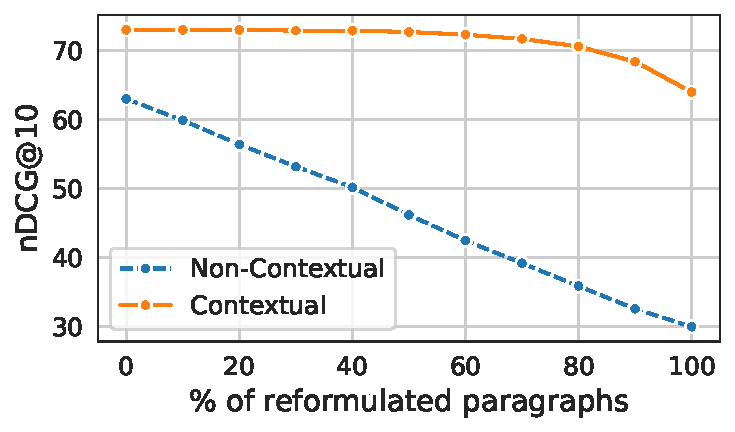
\includegraphics[width=0.65\textwidth]{images/conteb_images/reformulated.pdf}
    \caption[Importance of contextual information]{\textbf{Importance of Contextual Information:} Starting from a set of queries and mostly self-contained document paragraphs from the \emph{Football}, we progressively reformulate paragraphs to remove information redundant with the rest of the document. This leads to sharp performance declines in standard retrieval approaches, but not in contextual retrieval approaches.}
    \label{fig:reformulated}
\end{figure}

% In most applications, documents exhibit a highly structured format where individual paragraphs are not intended to be understood in isolation. Instead, they rely on prior context, document structure, or domain-specific knowledge. Acknowledging this is therefore necessary to incorporate all the relevant information into the representation of a passage.


\begin{figure*}[ht]
    \centering
    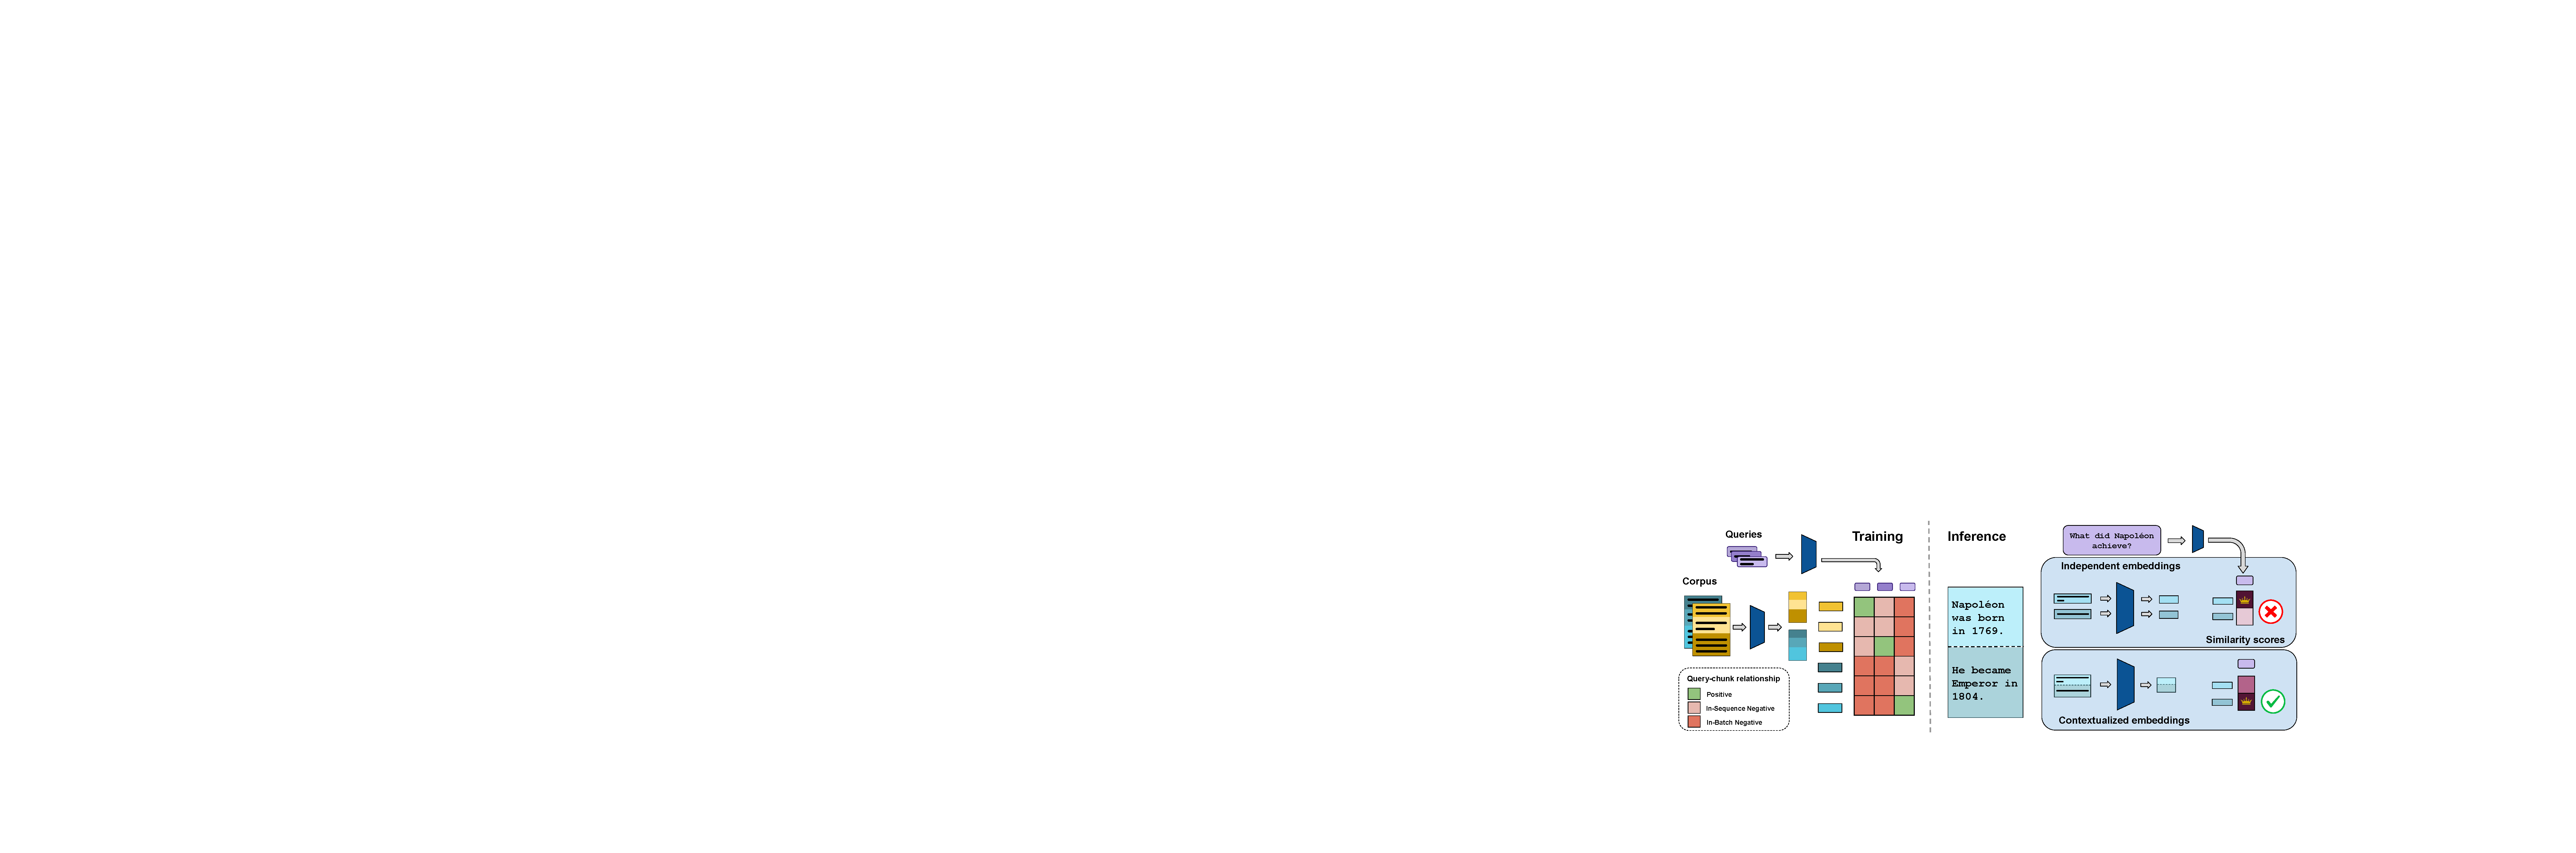
\includegraphics[width =\linewidth]{images/conteb_images/training_inference_final.pdf}
    \caption[Training vs inference overview]{
    \textit{Training (Left).} With respect to a single query, each chunk inside a batch plays a different role, depending on its original document, and the positive chunk.
    \textit{Inference (Right).} Traditional embedding methods (top) produce embeddings that do not include potentially essential contextual information. Contextualized embeddings (bottom) can integrate document-wide information in individual chunk representations, augmenting embedding relevance and improving downstream retrieval performance.}
    \label{fig:contextualized_exemple}
\end{figure*}

%\noindent\textbf{Industry Gap.} 
While long context encoders have been recently developed \sidecite{zhang2024mgte, modernbert, boizard2025eurobert} along with long context embedding models \sidecite{zhu2024longembedextendingembeddingmodels}, modern document retrieval pipelines typically segment lengthy documents into smaller chunks to optimize the granularity for efficient retrieval and readability of the retrieved content \sidecite{xu2024retrievalmeetslongcontext, jiang2024longragenhancingretrievalaugmentedgeneration}. Traditionally, these chunks are then \emph{independently} fed to an embedding model, and stored in a vector database for efficient future query matching. By doing so, these systems remove strong semantic and conceptual links between the split passages, directly affecting the resulting representations. An example is illustrated in \autoref{fig:contextualized_exemple}: embedding the sentence \textit{"He became emperor in 1804."} without leveraging information about the person at hand (\emph{Napoléon}) given in previous paragraphs will make matching queries related to \emph{Napoléon} difficult.

Recognizing the significant business value of incorporating broader contextual information into retrieval, major companies have explored leveraging large generative language models (LLMs) to mitigate this limitation. Some approaches attempt to circumvent retrieval altogether by feeding millions of tokens into the model's context window at runtime \sidecite{geminiteam2024gemini15unlockingmultimodal}, while others reformulate individual passages by concatenating them with document-level summaries and context \sidecite{contextual_anthropic}. However, these methods are prohibitively expensive at scale when dealing with corpora comprising thousands of documents.


%\noindent\textbf{Benchmarking.} 
Despite the critical importance of contextualized retrieval, standard benchmarks fail to capture this challenge. Evaluations traditionally focus on assessing the effectiveness of embedding models \sidecite{thakur_beir_2021, muennighoff_mteb_2022, saadfalcon2024benchmarkingbuildinglongcontextretrieval}, but they rely on datasets where document chunks are by design self-contained answer to the queries, which is a largely idealized scenario in practice \sidecite{thakur2025freshstackbuildingrealisticbenchmarks}. Consequently, benchmarks fail to highlight the limitations of current retrieval strategies in handling context-dependent passages. Worse, recent findings by \sidecite{zhou2025gsminfinitellmsbehaveinfinitely} indicate that some widely-used benchmarks exhibit biases that favor standard context-agnostic retrieval methods. Companies such as Anthropic have acknowledged these issues and maintain proprietary contextual retrieval benchmarks that remain unavailable to the public\sidenote{\url{https://www.anthropic.com/news/contextual-retrieval}}, underscoring the gap between academic evaluations and real-world industrial needs.

% To evaluate retrieval models, benchmarks such as BEIR \sidecite{thakur_beir_2021}, MTEB \sidecite{muennighoff_mteb_2022}, LoCo \sidecite{saadfalcon2024bencxhmarkingbuildinglongcontextretrieval} have been introduced, offering diverse real-world retrieval tasks. However, in practical settings, additional structural priors exist within the corpus providing information beyond mere document contents.


%
% Queries are generated for targeted passages, which results in scenarios where understanding the big picture of a document is unnecessary to correctly assign a chunk to its corresponding query. We aim at overcoming this pitfall by carefully crafting context-oriented evaluation samples.


% Other variant for the above sentence: Query-passage pairs are generated in such a way that understanding the big picture of a document is unnecessary to correctly assign a chunk to its corresponding query.
% While evaluations of document retrieval systems have traditionally focused on assessing embedding model quality \sidecite{thakur_beir_2021, muennighoff_mteb_2022}, they often neglect an important reality: document chunks are not independent - in practice, chunks most often originate from structured documents where information is naturally ordered and contextually linked. --> rephrased this
% Ignoring these relationships can lead to suboptimal retrieval performance, particularly when a chunk lacks sufficient context to be fully understood.

%In this work, we focus on evaluating retrieval systems on their capacity to efficiently leverage contextual information to construct meaningful chunk representations.

\noindent\textbf{Contribution 1: \textit{ConTEB}.}  
We introduce the \emph{Context-aware Text Embedding Benchmark}, designed to assess the ability of retrieval systems to leverage information from the entire document when indexing and retrieving document chunks. \emph{ConTEB} comprises both custom-designed tasks for fine-grained analysis, and practical retrieval evaluation settings spanning multiple document types, domains, and situations in which leveraging context is helpful to produce more meaningful chunk representations. 
We evaluate standard embedding methods on the benchmark and find they struggle when contextual awareness is required, while highlighting the promising contextual capabilities of approaches such as \emph{Late Chunking} \sidecite{LateChunking}.

\noindent\textbf{Contribution 2: \textit{Efficient Contextual Training}.}  
Improving upon the \textit{Late Chunking} method \sidecite{LateChunking}, we propose a novel embedding post-training method that optimizes information propagation between same-document chunks at indexing time to ensure embeddings are better contextualized. Our method largely boosts performance on \emph{ConTEB} %\textcolor{red}{over both non-contextual and training-free baselines, }
with minimal computational overhead. 
Through extensive ablations, we detail critical design choices and show our method displays increased robustness to sub-optimal chunking strategies and produces representations that scale better with corpus size. 

We open-source all project artifacts, including the benchmark, models and training data\sidenote{ \url{https://github.com/illuin-tech/contextual-embeddings}}.

% Document Retrieval consists in matching a user query to relevant documents in a given corpus. It is central to many industrial applications, either as a standalone ranking system (search engines) or as part of more complex information extraction or Retrieval Augmented Generation (RAG) pipelines. \manu{rephrase here, this is the colpali intro}

% \manu{briefly describe the process of indexing documents}
% Modern document retrieval pipelines often involve several phases; given a corpus of documents to index, a text extraction phase must first be conducted, in which documents will be parsed and chunked into a series of "chunks" of reduced length. These chunks are dimensioned to be short enough to XXX ([readable by a human, not exceeding context size, rag systems], yet they should ideally be of sufficient size to contain enough information to be somewhat self-contained thus providing  useful context to respond to a user's query.
% These chunks are then fed independently to text embedding models to obtain a vectorized chunk representation, which are stored in a vector database. Assessing the performance of document retrieval systems has historically most often been considered through the lens of embedding model evaluation. These evaluations are designed without consideration for the fact chunks are not independant and we may have priors on the corpus (such as the reading order in which to consider the chunks, the ones that come from the same document, their context, their amount, etc).

% In this paper, we focus on a main failcase of embedding models, which is when a chunk lacks sufficient conytext to be understood. 
% % cite the figure


% \begin{figure}
%     \centering
%     \includegraphics[width = 0.45\textwidth]{images/conteb_images/contextualized_example.png}
%     \caption{\manu{{Temporary placeholder figure}}}
    
%     % Latencies indicated in the figure are computed on the same machine \code{g2-standard-16} with a NVIDIA-L4 GPU, and averaged over 100 pages. Further details in \autoref{subsection:latency}.The computed score is the average of from all datasets in \textit{ViDoRe} for PDF Parser + Captioning and ColPali respectively. Further details in \autoref{section:results}.} 
%     \label{fig:contextualized_exemple}
% \end{figure}


% In this work, we focus on integrating contextual information into a given passage's latent representation.


% \noindent\textbf{Contribution 1: \textit{Context-aware embedding evaluation}.}
% We propose CAEEL, the Context-aware embedding evaluation Leaderboard, a series of retrieval-oriented tasks spanning multiple document types and domains \manu{and languages ?} that aims to assess the capacity of a retrieval system to leverage prior contextual information about passages in the construction of their embeddings. We show current top models struggle.

% \noindent\textbf{Contribution 2: \textit{In-sequence negative training strategy}.}
% Leveraging recent advances in long-context encoder models, and extending work on late chunking, we propose a novel modeling and training approach to seamlessly integrate context in passage representations with very little compute overhead. We show our approach, consisting of training with in-sequence negatives, is well aligned with standard retrieval applications and boosts performance. Our codebase which we openly release is model agnostic and is compatible with all sentence-transformers embedding models.



% \textbf{Contribution 4.}
% We release our fine-tuned models and training code under open licenses, bringing to both researchers and industry practitioners state-of-the-art document retrieval models\sidenote{\url{hf.co/anon}}. We also release all artifacts related to benchmarking\sidenote{\url{github.com/anon}} (data, evaluation code, public leaderboards, reproducible baselines) to serve as a new reference for Document Retrieval.



% \noindent\textbf{Problem Setting.}
% In our setting, a retrieval system scores how relevant a document $d$ from corpus 
% \manu{add math}

% Neural embedding models to represent texts at a passage level were introduced by \sidecite{reimers2019sbert} \manu{little history recap}. \manu{mention synthetic data, infonce, late interaction}. Long context models.

% To evaluate such models \manu{beir, mteb}.In practice, much more priors exist on the data distribution within the corpus. \manu{add math to show we have knowledge of D in its entirety often times, and metadata that enables us to have a stucture on D.} Long context evaluation.

% Modern  techniques have been developped to compensate for the incapacity of embedding models to integrate knowledge beyond their passage scope. \manu{mention smart chunking techniques + contextual embeddings antrhropic, raptor, graph rag}

% All these techniques however either necessitate heavy intervention of external LLMs (reformuation), are hard to scale to large corpora, or are very brittle and based on carefully crafted heuristics or document parsing approaches (chunking) which have been shown to be suboptimal [CITE].


% \noindent\textbf{Late Chunking.} Late chunking is a training-free pooling token pooling technique \manu{add math about late chunking} Authors have designed the method to be able to reduce the chunk size while maintaining strong performance. We are interested in seeing whether through training we can induce better information propagation and optimize the method...

\section{Problem Formulation \& Related Work}

% \subsection{Problem statement}
% As illustrated in \autoref{fig:contextualized_exemple}, embedding models that disregard document-level context often lack crucial information. In the example, the pronoun "They" refers to an entity mentioned earlier, which must be resolved to ensure correct chunk embeddings for queries about the Brazilian Football team. More broadly, retrieval systems integrate with document ingestion pipelines, leveraging metadata such as document membership and chunk position. This work explores utilizing these priors to enhance retrieval in context-dependent scenarios.

%M In standard retrieval pipelines, long documents are chunked and independently processed by an embedding model. 
% \pierre{embeddings that do not leverage contextual information from the chunking step will lack of essential information : ici je reciterais la figure 1 du dessus}

% \subsection{Contextual chunk representation}
% \manu{Probably remove this entire paragraph, or change with figure 2.} As illustrated in \autoref{fig:reformulated}, embedding models that do not consider document-level knowledge ("context") will often lack essential information when producing a chunk representation. In the illustration (\autoref{fig:contextualized_exemple}), the pronoun \textit{"They"} in the second chunk is ambiguous without context. Retrieval models that are able to leverage contextual information will have a much easier time matching this chunk to queries about either Brazilian football or Napoleon. Generally, it is straightforward to inject contextual information such as the source document, or the position of the chunk within it. Systematically incorporating these priors to improve retrieval is the focus of this work.

\subsection{Retrieval Frameworks}
In this paper, we consider the traditional retrieval framework where a retrieval system given a query \(q\), searches a corpus \(\mathcal{D}\) for relevant documents. Each document \(d \in \mathcal{D}\) is scored based on its content by first embedding the text into a vector space, and then computing a similarity measure. The similarity between a query \(q\) and a document \(d\) is defined as
\begin{equation}
\text{sim}(q, d) = f\big(\phi(q), \phi(d)\big) \nonumber
\end{equation}
where \(\phi\) maps text into an \(n\)-dimensional vector space and \(f: \mathbb{R}^n \times \mathbb{R}^n \to \mathbb{R}\) is a similarity function, such as cosine similarity or dot product.

In applied settings, individual documents are often too long to be practical for retrieval purposes \sidecite{Liu_LlamaIndex_2022, mixofgranularity}. % \manu{expand and illustrate}
Each document \(d\) is thus divided into segments called \emph{chunks} by a partitioning function \(\mathcal{P}\) defined as
\begin{equation}
\mathcal{P}(d) = \{c_1, c_2, \dots, c_{N_d}\} \nonumber%, d = \bigcup_{i=1}^n c_i \nonumber
\end{equation}


% with each chunk \(c_i\) representing a segment of \(d\) and $N_d$ represents the number of chunks in the document $d$.

% The complete set of metadata across the corpus is given by
% \[
% M = \{M_c \mid c \in \mathcal{D}\}.
% \]
% The retrieval function \(\text{sim}(q, c)\) assigns a relevance score to a query \(q\) and a chunk \(c\). 
In the \emph{standard retrieval} setting, the score is computed solely based on chunk content:

\begin{equation}
\text{sim}(q, c) = f\big(\phi(q), \phi(c)\big) \nonumber
\end{equation}

 Additional information (priors) is however often available to the document embedding system. Typically, knowledge of the entire corpus $\mathcal{D}$, or of \emph{structural metadata} \(M_c\) such as neighboring document chunks obtained through \(\mathcal{P}\), can be leveraged by a modified embedding function \(\phi_2\), yielding the following similarity score:
\begin{equation}
\text{sim}(q, c) = f\Big(\phi(q), \phi_2\big(c, M_c, \mathcal{D}\big)\Big) \nonumber
\end{equation} 

\noindent\textit{This work is centered on efficiently integrating priors about the entire document when embedding a sub-document chunk.}


% \noindent\textbf{Problem Setting.} In our setting, a retrieval system assigns a relevance score to a document $d$ from a corpus $\mathcal{D}$ given a query $q$. Typically, this involves computing a similarity function $\text{sim}(q, d)$ using dense or sparse representations:
% \begin{equation}
% \text{sim}(q, d) = f(\phi(q), \phi(d))
% \end{equation}
% where $\phi$ is an embedding function that maps text into a vector space, and $f$ measures similarity, commonly using cosine similarity or dot product.

% Let $\mathcal{D}$ denote a corpus composed of multiple documents $d \in \mathcal{D}$, where each document $d$ is further composed of multiple chunks $c \in d$. The chunking process is defined by a partition function $\mathcal{P}$ such that:
% \begin{equation}
%     \mathcal{P}: d \to \{c_1, c_2, \dots, c_n\}, \quad \forall d \in \mathcal{D}, \quad c_i \in d.
% \end{equation}

% As the retrieval system itself often handles this decomposition,  the additional structural priors, including the fact that chunks originate from the same document and their relative positions within that document are known and usable by the system during indexing. We denote this metadata information by $M = \{M_c \mid c \in \mathcal{D}\}$, where $M_c$ includes document membership and ordering constraints.

% The retrieval function $S(q, c)$, which assigns a relevance score to a query $q$ and a chunk $c$, can be defined in two settings:

% \noindent\textbf{Standardly}: The retrieval model assigns a score based purely on content similarity:
%    \begin{equation}
%        \text{sim}(q, c) = f(\phi(q), \phi(c))
%    \end{equation}
%    where $f(q, c)$ is a function of the semantic similarity between the query and the chunk, typically computed via dense embeddings or lexical matching.

% \noindent\textbf{With Structural Priors}: The scoring function incorporates metadata $M_c$, allowing it to leverage document structure:
%    \begin{equation}
%        S(q, c) = f(\phi(q), \phi_2(c, M_c, \mathcal{D})
%    \end{equation}
%    where $M_c$ contains structural priors such as inter-chunk relationships, document cohesion, and positional significance.


\subsection{Integrating Contextual Information} \label{related_work_contextual}
Neural embedding models for passage-level text representation, popularized by SentenceBERT \sidecite{reimers2019sbert}, have enabled retrieval systems to move beyond lexical matching \sidecite{robertson_okapi_1994}. To include contextual information in these retrievers, previous works proposed methods that either operate \textit{offline} during \emph{indexing}, or online during \emph{querying} when faced with a user request.

\noindent\textbf{Indexing.} The chunking strategy is a crucial design choice and often aims to optimize chunk self-containment. Fixed-size approaches with overlaps preserve continuity, while structure-aware chunking respects natural text boundaries, such as paragraphs or sentences. Semantic chunking, by contrast, splits text into topic-aligned segments. These methods appear in frameworks such as LlamaIndex \sidecite{Liu_LlamaIndex_2022} and LangChain \sidecite{chase_langchain_2022}, but different queries may need different chunk sizes. Thus, dynamic chunking techniques have emerged to adapt segmentation on the fly \sidecite{mixofgranularity, qian2024groundinglanguagemodelchunkingfree}. Beyond optimizing chunking, some indexing approaches enrich chunks with broader context by preprending LLM-generated document summaries, contextual information or metadata \sidecite{contextual_anthropic, multimetarag}. Similarly, \sidecite{morris2024contextualdocumentembeddings} demonstrate that appending learned "corpus" embeddings to queries and documents can further improve retrieval. Other indexing-time techniques involve organizing chunks into higher-level data structures. For example, \sidecite{graphrag} and \sidecite{raptor} cluster related chunks into semantic graphs or tree hierarchies.

%\textcolor{red}{\sidecite{LateChunking} introduced the \textit{Late Chunking} paradigm, which leverages the large context window of embedding models to enable cross-chunk information propagation, yielding small improvement gains on standard retrieval datasets, hinting at chunk contextualization potential.}

\noindent\textbf{Querying.} In contrast, \emph{query-time} solutions rely on iterative or agentic loops to refine retrieval dynamically. LLMs can be used to iteratively update the query or request additional chunks based on partial results \sidecite{MultiHopRAG, IrCoTRAG}, or even to run “self-checks” and seek extra context when needed \sidecite{selfrag}. While these adaptive techniques can better address complex, multi-hop queries, they typically require much more computational resources during inference.

% \manu{rewrite} In this paper we propose a method to efficiently leverage document-level contextual information during indexing without the need for external LLMs and with no computational overhead.


%\subsection{Integrating contextual information}



% \manu{here restructure}
% Neural embedding models for passage-level text representation were popularized with SentenceBert \sidecite{reimers2019sbert}, enabling semantic search beyond traditional lexical matching \sidecite{robertson_okapi_1994} have been widely adopted to train embedding models in retrieval tasks. 

% \subsection{Integrating contextual information.}
% \label{related_work_contextual}


% \manu{Restructure as indexing vs querying time approaches}

%The document partitioning process \(\mathcal{P}\) is crucial in optimizing the performance of retrieval systems. Chunks must strike a balance between two competing constraints: \textit{compactness} and \textit{self-containment}. They should be short enough to remain readable and fit within the context window of modern language models, but each chunk should also include enough contextual information to be interpretable on its own, reducing reliance on other parts of the document.

%Refining chunks to get the most suitable representations
% Building a context-aware retrieval system is a complex problem that can be tackled at different levels. Some solutions are implemented offline at document ingestion and indexing time,
%- refining chunks to get the most suitable representations - 
% while others trade inference time with elaborate retrieving algorithms to make sure that the relevant chunks can be found.

%\manu{simplify, add citations}
% \noindent\textbf{Optimizing Chunking.} 
% Effective chunking strategies are essential for optimal performance in language models. Commonly adopted approaches include structure-aware chunking, attempting to keep paragraphs and sentences together, and semantic chunking, splitting text based on meaningful units with similar topics. These techniques are found in the popular and widely used implementation frameworks \sidecite{Liu_LlamaIndex_2022, chase_langchain_2022}.
%Common approaches include fixed-size chunking, where text is divided into uniform segments with possible overlaps to maintain context continuity, Structure-Aware chunking where chunks attempts to keep paragraphs and sentences together, and semantic chunking, splitting text based on meaningful units with similar topics. All of these techniques are found in the popular and widely used implementation frameworks \sidecite{Liu_LlamaIndex_2022, chase_langchain_2022}.
%, ensuring each chunk conveys a complete idea
% However, there is no one-size-fits-all solution since the optimal granularity of the chunk depends directly on the query at hand, which motivated dynamic chunking methods \sidecite{mixofgranularity, qian2024groundinglanguagemodelchunkingfree}.
% Hybrid chunking combines both methods, adjusting chunk sizes dynamically to balance readability and context preservation. These strategies aim to create chunks that are both manageable for processing and rich in information, facilitating more accurate and efficient retrieval. --> maybe no need to expand on hybrid approaches as we don't have specific examples to cite

% \noindent\textbf{Context Infusion.} Some approaches leverage the long-context capabilities of LLMs to refine chunks by incorporating broader context in the form of concatenated text \sidecite{contextual_anthropic} and metadata \sidecite{multimetarag}, leading to improved retrieval performance at higher corpus ingestion costs. Concatenating corpus-level vector representations to queries and documents before feeding them to an embedding model \sidecite{morris2024contextualdocumentembeddings} has also been shown to yield performance improvements. 

%Enhancing chunk representations can be achieved by employing large language models (LLMs) that access document-wide information. By incorporating broader context in the form of concatenated text \sidecite{contextual_anthropic} and metadata \sidecite{multimetarag}, these approaches leverage the long-context capabilities of LLMs to generate more accurate and relevant representations of chunks, leading to improved retrieval performance at higher corpus ingestion costs. Techniques such as concatenating corpus-level representations to query and document token embeddings \sidecite{morris2024contextualdocumentembeddings} have also been shown to yield performance improvements.

% (reformulated above) This approach, known as contextual retrieval, utilizes techniques like contextual embeddings and contextual BM25 to improve the retrieval step in retrieval-augmented generation (RAG) systems. By incorporating broader context, LLMs can generate more accurate and relevant representations of chunks, leading to improved retrieval performance. 

% \noindent\textbf{Structured Corpus Representation.} Organizing documents into a data structure is yet another approach that aims at improving retrieval. At ingestion time, chunks can be assembled into structures such as graphs \sidecite{graphrag} or trees \sidecite{raptor} based on their semantic similarity, often with the help of LLMs. These methods leverage the structured relationships between entities to provide more comprehensive and contextually relevant information during retrieval.
%, enhancing the overall performance of the system. 

%\noindent\textbf{Graph-Enhanced Retrieval.} Incorporating document relationships, such as citation graphs, into retrieval processes can significantly improve quality. GraphRAG, for instance, integrates knowledge graphs and graph databases with traditional retrieval-augmented generation techniques. This method leverages the structured relationships between entities to provide more comprehensive and contextually relevant information during retrieval, enhancing the overall performance of the system. 

% \noindent\textbf{Inference-Time Approaches.} LLMs can be used in agentic loops to iteratively refine queries and improve retrieval quality. Complex pipelines \sidecite{selfrag, MultiHopRAG, IrCoTRAG} involve the LLM over multiple steps, evaluating iteratively whether additional chunks should be retrieved. 

% \noindent\textbf{Inference-Time Approaches.} LLMs can be used in agentic loops to iteratively refine queries and improve retrieval quality. \sidecite{selfrag} employs the generations to trigger and evaluate the retrieval mechanism, while SeaKR \sidecite{SeaKR} does so using the LLM internal states. Multi-hop approaches \sidecite{MultiHopRAG, IrCoTRAG} involve the LLM over multiple steps, evaluating iteratively whether additional chunks should be retrieved. 
% At inference time, advanced strategies like self-retrieval augmented generation (Self-RAG) and multi-hop retrieval are employed to enhance performance. Self-RAG involves the model retrieving and utilizing its own generated content to refine answers, while multi-hop retrieval allows the model to gather information from multiple related documents or chunks to answer complex queries. These methods aim to reduce computational overhead and improve scalability by minimizing reliance on external interventions and heuristics.

% Despite their success, these methods often rely on computationally expensive LLMs either during indexing or querying, and are impractical to scale to larger corpora.
% \manu{mention late chunking}


\section{\textit{ConTEB}: Context-aware Text Embedding Benchmark}


% \section{\textit{ConTEB}: Context-Aware Embedding Leaderboard}
\label{section:loco_benchmark}

% \manu{This section needs to highlight the fact that existing datasets are not adapted, nor easily adaptable for our tasks. There is a real "extractive" bias in existing datasets which causes questions to be super extractive and often self contained.}




\begin{comment}
\begin{table*}[h]
    \centering
    \scriptsize
\resizebox{\linewidth}{!}{
    \begin{tabular}{lcc|cc}
    \toprule
     & Chunk Annotation & Verification & Domain & Context requirement type \\
    \midrule
    \vspace{1mm}\textbf{In Domain} & \\
    MLDR & Synthetic & & Encyclopedic & Document-level reasoning \\
    NarrativeQA & Synthetic & & Literature & Document-level reasoning \\
    SQuAD & Manual & & Encyclopedic & Chunk not self-contained  \\
    \midrule
    \vspace{1mm}\textbf{Out-Of-Domain} & \\
    Footballers & By design & \darkgreencheck  & Sports & Co-reference resolution \\
    Geography & By design & \darkgreencheck & Geography & Co-reference resolution \\
    Insurance & By design & \darkgreencheck & Insurance & Structure understanding \\
    Covid-QA & Synthetic & & Medical & Chunk not self-contained \\
    ESG Reports & Manual & & Industry  & Context disambiguation \\
    NanoBEIR* & Manual & & Varied & - \\
    \bottomrule
    \end{tabular}
    }
  \captionof{table}{ConTEB details}
  \label{tab:conteb_details}
\end{table*}
\end{comment}


\begin{comment}
\begin{table}
    \centering
    \scriptsize
    \resizebox{\linewidth}{!}{%
    \begin{tabular}{lcccc}
    \toprule
     & Pairing & Verification  \\
    \midrule
    \vspace{1mm}\textbf{In Domain} & \\
    MLDR & Synthetic &  & \\
    NarrativeQA & Synthetic &  \\
    SQuAD & Existing &  \\
    \midrule
    \vspace{1mm}\textbf{Out-Of-Domain} & \\
    Footballers & By design & \darkgreencheck \\
    Geography & By design & \darkgreencheck \\
    Insurance & By design & \darkgreencheck \\
    Covid-QA & Synthetic &  \\
    ESG Reports & Manual &  \\
    NanoBEIR* & Existing &  \\
    \bottomrule
    \end{tabular}
    }
    \label{tab:example}
    \captionof{table}{Example table}
\end{table}
\end{comment}


% LaTeX code for a compact ConTEB statistics table (no zebra striping)
% Required packages (add to your preamble if not already present):
%   \usepackage{booktabs, siunitx, xcolor, colortbl, multirow, graphicx, array}
%   \sisetup{detect-all}

\begin{table*}[ht]
  \centering
  \small

  % ------- siunitx column configuration (slightly narrower) -------
  \sisetup{
    table-number-alignment = center,
    table-figures-integer  = 4,
    table-figures-decimal  = 1,
    table-column-width     = 12mm,
  }

  % ------- custom colors for group labels -------
  \definecolor{grpA}{HTML}{C6E0FF}   % In-Domain background
  \definecolor{grpB}{HTML}{FFD6D6}   % Out-of-Domain background

  % ------- helper for fixed-width first column (vertical labels) -------
  \newcolumntype{C}[1]{>{\centering\arraybackslash}p{#1}}

  % ------- slightly larger rows to fit sentences -------
  \renewcommand{\arraystretch}{1.25}

  \begin{tabular}{
      C{5mm}                          % Domain group (fixed width, centered)
      l                                % Dataset name
      S[table-format=3.1]                % # Queries
      S[table-format=3.1]                % # Docs
      S[table-format=3.1]              % Tokens / Chunk
      S[table-format=3.1]              % Chunks / Doc
      c
      % p{40mm}                          % 5-word sentence (fixed width)
  }
  \toprule
   & Dataset & {Queries} & {Docs} & {\shortstack{Tokens per\\[-1pt]Chunk}} & {\shortstack{Chunks per\\[-1pt]Document}}  & {Context Utilization} \\
  \midrule
  % ---------------- In-Domain ----------------
  \multirow{3}{*}{{\rotatebox[origin=c]{90}{\shortstack{\textbf{In}\\[-1pt]\textbf{Domain}}}}}
    & MLDR      &  100 &  100 & 170.5 & 15.4 & Document-level reasoning \\
    & NarrativeQA       & 8575 &  355 & 154.5 &  4.9 & Document-level reasoning   \\
    & SQuAD     & 2067 & 2067 &  19.1 &  8.5 & Chunk not self-contained \\
  \midrule
  % -------------- Out-of-Domain --------------
  \multirow{6}{*}{{\rotatebox[origin=c]{90}{\shortstack{\textbf{Out of}\\[-1pt]\textbf{Domain}}}}}
    & {\color{navyblue}\textbf{Football}}   & 2682 & 301 &  77.4 &  20.8 & Co-reference resolution \\
    & {\color{navyblue}\textbf{Geography}}  & 5283 &  530 & 113.6 &  4.3 & Co-reference resolution     \\
    & {\color{navyblue}\textbf{Insurance}}  &  120 &    1 &  80.7 & 60.0 & Structure understanding \\
    & Covid-QA            & 1111 &  115 & 153.9 & 29.1 & Chunk not self-contained  \\
    & ESG Reports         &   36 & 30 & 205.5 & 123.4 & Context disambiguation \\
    & NanoBEIR$^*$        &  650 & 56723 & 199.4 &  1 & No context is needed  \\
  \bottomrule
  \end{tabular}

  \caption[ConTEB dataset details]{Merged \emph{ConTEB} dataset details. Controlled datasets are highlighted in {\color{navyblue}\textbf{bold blue}}. NanoBEIR values are summed over the 13 datasets that compose it.}
  \label{table:merged_conteb}
\end{table*}

%      & Chunk Annotation & Verification & Domain & Context requirement type \\
%     \midrule
%     \vspace{1mm}\textbf{In Domain} & \\
%     MLDR & Synthetic & & Encyclopedic & Document-level reasoning \\
%     NarrativeQA & Synthetic & & Literature & Document-level reasoning \\
%     SQuAD & Manual & & Encyclopedic & Chunk not self-contained  \\
%     \midrule
%     \vspace{1mm}\textbf{Out-Of-Domain} & \\
%     Footballers & By design & \darkgreencheck  & Sports & Co-reference resolution \\
%     Geography & By design & \darkgreencheck & Geography & Co-reference resolution \\
%     Insurance & By design & \darkgreencheck & Insurance & Structure understanding \\
%     Covid-QA & Synthetic & & Medical & Chunk not self-contained \\
%     ESG Reports & Manual & & Industry  & Context disambiguation \\
%     NanoBEIR* & Manual & & Varied & - \\
%     \bottomrule
%     \end{tabular}
%     }
%   \captionof{table}{ConTEB details}
%   \label{tab:conteb_details}
% \end{table*}


\subsection{Benchmark Design}

Existing benchmarks often rely on (or assume) self-contained document chunks. This creates a misleading perception that contextualization offers little to no benefit, which in practice is rarely the case. To address this gap, the \emph{ConTEB} benchmark philosophy is to explicitly be composed of tasks in which leveraging document-wide context should lead to performance improvements. Our benchmark originates from two sources: new datasets specifically created for \emph{ConTEB}, and repurposed academic datasets. We take special care in selecting data sources spanning from multiple domains, including realistic industrial scenarios.

\noindent\textbf{Why Context?} Context can help resolve ambiguity, such as distinguishing between multiple meanings of a word or resolving pronouns and entity references (co-reference resolution). It is crucial when documents have a structured format, like legal or scientific texts, where understanding table of content hierarchy is key to aid intra-document disambiguation. Inversely, document-level contextual information is key when querying a corpus of documents that follow a strongly similar structure, such as annual company reports, to enable cross-document disambiguation.

% We mix both tasks designed specifically to elicit context, and existing academic datasets repurposed for \emph{ConTEB}. Furthermore, we take special care in selecting data sources spanning from multiple domains, including realistic industrial scenarios.

% In our benchmark, retrieval performance is measured in scenarios where naive chunk-based approaches fail. By evaluating systems under these structured conditions, we provide a clearer picture of how well retrieval systems leverage context, rather than merely optimizing for chunk-level similarity.



% This enables the benchmark to cover an array of situations.
% \begin{table}[h]
%     \centering
%     \scriptsize
% \resizebox{\linewidth}{!}{
%     \begin{tabular}{lcc}
%     \toprule
%      & Domain & Context requirement type \\
%     \midrule
%     \vspace{1mm}\textbf{In Domain} & \\
%     MLDR & Encyclopedic & Document-level reasoning \\
%     NarrativeQA & Literature & Document-level reasoning \\
%     SQuAD & Encyclopedic & Chunk not self-contained  \\
%     \midrule
%     \vspace{1mm}\textbf{Out-Of-Domain} & \\
%     \textcolor{navyblue}{\textbf{Sports}} & Sports & Co-reference resolution \\
%     \textcolor{navyblue}{\textbf{Geography}} & Geography & Co-reference resolution \\
%     \textcolor{navyblue}{\textbf{Insurance}} & Insurance & Structure understanding \\
%     Covid-QA & Medical & Chunk not self-contained \\
%     Vidore-ESG Reports& Industry  & Context disambiguation \\
%     \bottomrule
%     \end{tabular}
%     }
%   \captionof{table}{\emph{ConTEB} constitution details. Controlled datasets are highlighted in \textcolor{navyblue}{\textbf{bold blue}}. The other datasets are stemming from academic benchmarks and repurposed for \emph{ConTEB}.}
%   \label{table:conteb_details}
% \end{table}

% \subsection{Benchmark Construction}
% \label{sec:bench-construction}

\noindent\textbf{Concept.} To isolate the importance of contextual cues and diminish other confounding factors, we construct three benchmark tasks to study contextualization in controlled experimental settings \sidecite{AllenZhu-icml2024-tutorial}. 
% By design, we ensure leveraging context is useful for these tasks. 
We also evaluate more practical retrieval settings at larger scale where we suspect contextualization to help, and in which we rely on organic, pre-existing query-document pairs.

\subsection{Benchmark Construction} 
%\begin{comment}
\begin{figure*}[htbp]
  \centering
  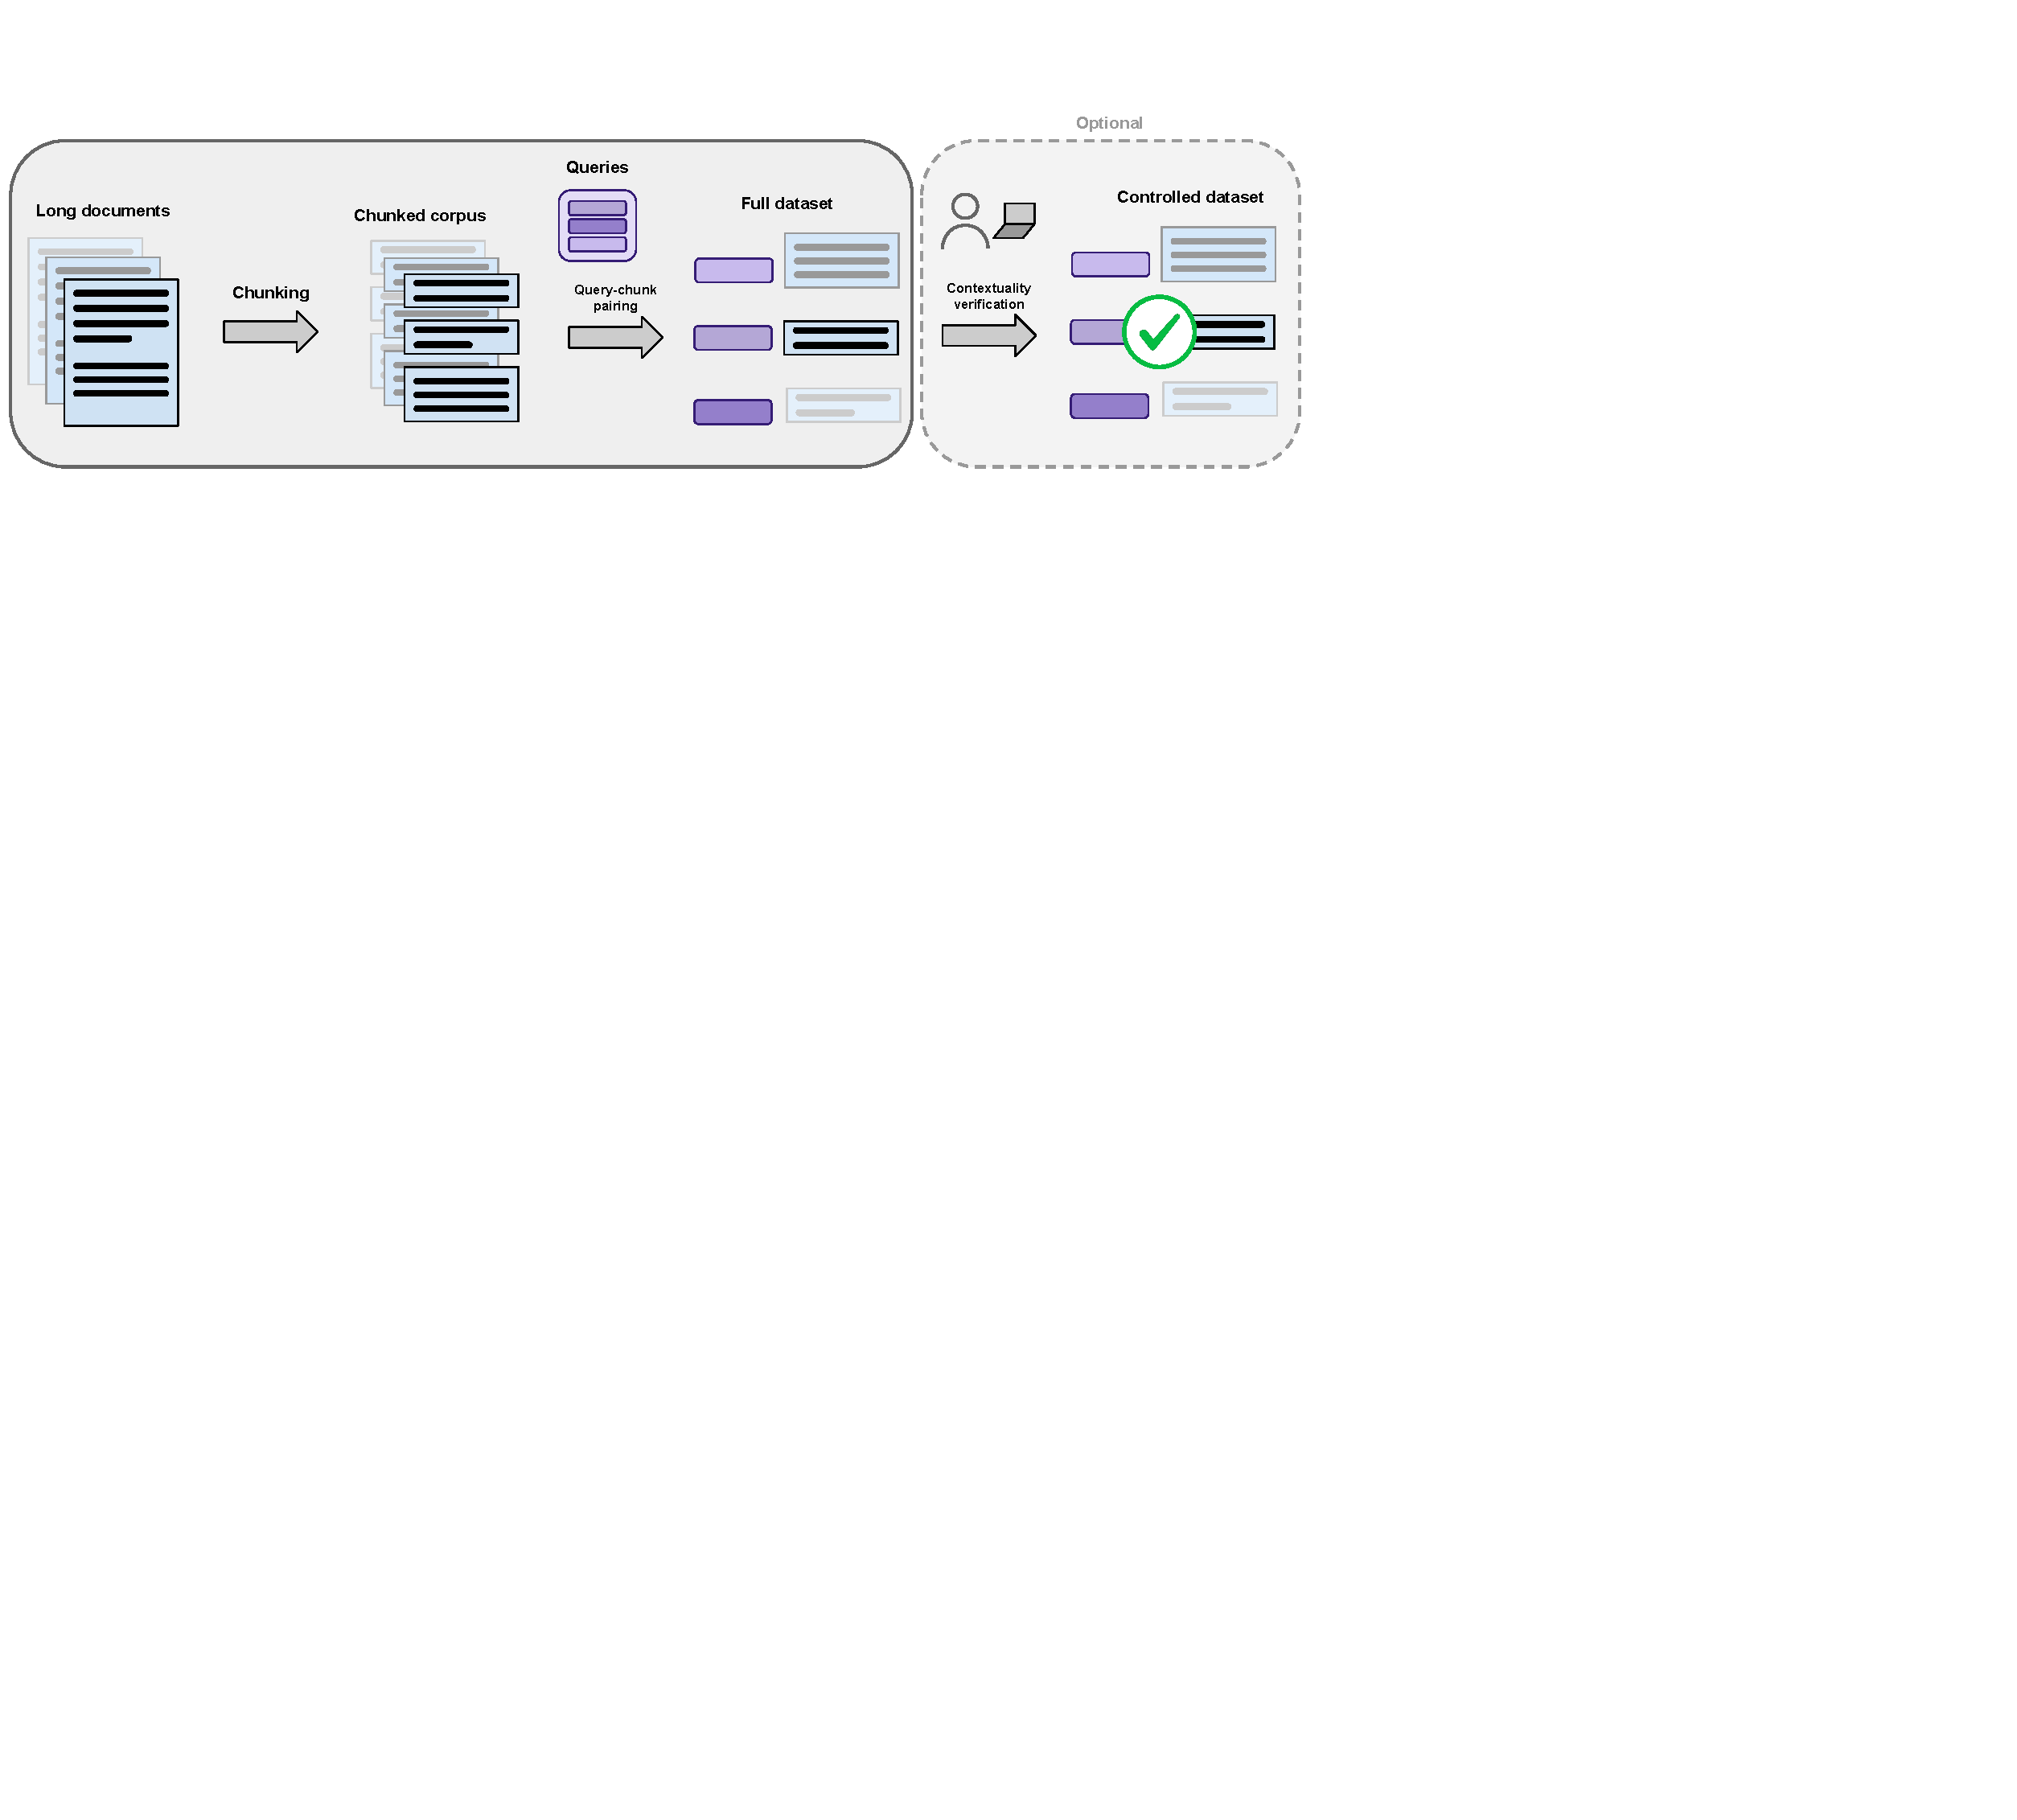
\includegraphics[width=1.3\textwidth]{images/conteb_images/benchmark_creation_horizontal.pdf}
  \caption[Benchmark creation process]{Benchmark creation process.}
  \label{fig:benchmark_creation}
\end{figure*}

% \textcolor{red}{ADD RELEVANT DETAILS FROM APPENDIX}
% Our generic benchmark curation pipeline is composed of three stages. 
% \textcolor{red}{Depending on the existing data at hand, each stage is applied slightly differently across all datasets.}
% We provide additional curation details in \autoref{app:conteb_stats}. 
% \textcolor{red}{
The generic dataset curation pipeline is depicted in \autoref{fig:benchmark_creation}. This three-stage process allows us to obtain queries linked to chunks belonging to long documents, that contain context with respects to each chunk. We apply this pipeline to each of our data sources, with minor adjustments depending on the existing data at hand, that we detail in \autoref{app:conteb_stats}. 
%In particular, we apply the optional stage of the pipeline to create our controlled setup.}

\noindent\textbf{1: Chunking.} We select long documents spanning a variety of domains and chunk them through a structure-aware method\sidenote{RecursiveCharacterSplitter with a threshold of 1000 characters \cite{chase_langchain_2022}} \sidecite{rajpurkar-etal-2016-squad, moller-etal-2020-covid, kočiský2017narrativeqareadingcomprehensionchallenge, chen_bge_2024, macé2025vidorebenchmarkv2raising}.

\noindent\textbf{2: Pairing.} 
%For datasets for which queries related to the longer original document are available, we associate them to the most relevant chunk(s) using existing manual annotations (SQuAD, ESG), or a large language model (CovidQA, MLDR, NarrativeQA). 
We use manual answer span annotations (\emph{SQuAD}, \emph{ESG}) or synthetically label them with a LLM (\emph{CovidQA}, \emph{MLDR}, \emph{NarrativeQA}), to match queries with chunks obtained in Stage 1. This ensures queries are not solvable by design \sidecite{thakur2025freshstackbuildingrealisticbenchmarks}. Alternatively, in our controlled experiment tasks, we generate queries pertaining to the chunks manually (\emph{Insurance}) or synthetically using LLMs (\emph{Football}, \emph{Geography}).


\noindent\textbf{3: Manual Verification \& Modification.}
%Sabotage.
The manually crafted questions in \emph{Insurance} are designed to be ambiguous without prior knowledge of the document structure. This is manually verified in this phase. Going a step further, in \emph{Football} and \emph{Geography}, we reformulate chunks with the help of a LLM to remove explicit mentions of the original document's theme which all queries mention. We do so in all but the first chunks of each document, explicitly enforcing the need for context.

In addition to our contextual scenarios, we use \emph{NanoBEIR} \sidecite{thakur_beir_2021} to evaluate non-regression on standard non-contextualized embedding tasks.

% We apply the optional control stage of the pipeline to three datasets--\emph{Footballers}, \emph{Geography}, and \emph{Insurance}--in order to enforce inter-chunk contextual links, to extensively test the capabilities of contextualization methods. The other datasets are adopted academic datasets, that we repurpose to our task with our pipeline, thereby introducing contextualization challenges. 
% Table \ref{table:conteb_details} provides an overview of the covered domains and the context types across datasets.
%\end{comment}

\noindent\textit{By combining hard tasks in controlled environments, repurposed academic benchmarks, and real-world industrial queries, our benchmark provides a comprehensive assessment of retrieval models in both standard and context-dependent retrieval scenarios.}

\subsection{Training Dataset}

Open training data is a key factor to ensure fair comparison across methods and robust conclusion. In addition to our benchmark, we construct and release a training dataset composed of query and document chunk pairs. It includes the training splits of \emph{MLDR} and \emph{NarrativeQA}, repurposed with our previously detailed pipeline. To increase the number of queries, we further use \emph{GPT-4o} to generate relevant supplementary synthetic queries. We also concatenate \emph{SQuAD} chunks from the same Wikipedia article, keeping track of the original question-passage associations. 
The full dataset contains 9881 unique long documents (3698 tokens on average), corresponding to a total of 232'587 chunks and 307'241 queries (see \autoref{app:training_data}). Scaling the dataset to more sources, through diverse synthetic augmentations and refinement–based augmentation methods \sidecite{lee2024nvembedimprovedtechniquestraining, wang2024improvingtextembeddingslarge} is left for future work.


\subsection{Baselines}
% In addition to raptor, cde, contextual, 0-shot sentence transformers, we train sentence transformers with the same data (same batch) than whazt we train CDE on.

%\pc{Pour moi faut se positionner et dire pourquoi on pool au niveau de la sentnece.} More recently, approaches such as late interaction models \sidecite{khattab2020colbert, chen_bge_2024} and  gained in popularity, setting new performance standards for encoder-based models. \pc{cokokok}


\noindent\textbf{Training-Free.} We evaluate a selection of off-the-shelf methods that are strong in their size categories such as a standard single-vector embedding model based on ModernBERT (\texttt{modernbert-embed-large} \cite{modernbert, ModernBERT-embed-large}), its multi-vector ColBERT equivalent \sidecite{khattab2020colbert, GTE-ModernColBERT} and \emph{Okapi BM25} \sidecite{robertson_okapi_1994}, a strong lexical matching method. 
Additionally, we compare against various contextualization approaches. Specifically, we include Anthropic’s contextual retrieval approach~\sidecite{contextual_anthropic}\sidenote{We use \texttt{Qwen-2.5-7B-Instruct} as the generative model which we serve on a 80GB A100 GPU with vLLM and \texttt{modernbert-embed-large} as the embedding model}, and evaluate Late Chunking \sidecite{LateChunking} without specific fine-tuning using \texttt{modernbert-embed-large}. These methods cover standard practices with varying level of complexities and indexing budgets.\sidenote{We also evaluate RAPTOR \cite{raptor} with \texttt{Qwen-2.5-7B-Instruct} and \texttt{cde-small-v2}~\cite{morris2024contextualdocumentembeddings} but find them to be poorly adapted to our problem settings.}

\noindent\textbf{Training-Based.} For fair evaluation, we also fine-tune the sentence embedding method \texttt{modernbert-embed-large} on the training dataset with the same batch construction strategy as when training our main method, ensuring performance differences only stem from methodological design.

% Our baselines are separated into two main categories: different training methods applied to the same base models that we use, and different embedding contextualization approaches.

% \noindent\textbf{ModernBERT-based baselines}
% We evaluate 4 different settings for the same base model: the base model itself, a version fine-tuned on our training dataset but in a single-context manner, a version applying late chunking without training, and our full version ContextEmbed \maxou{find name}.

% \noindent\textbf{Different embedding techniques}
% We compare our models to a sample of the different contextualization approaches detailed in \ref{related_work_contextual}, including Anthropic's contextual retrieval \sidecite{contextual_anthropic} and RAPTOR \sidecite{raptor}. For these baselines, we use \texttt{Qwen-2.5-7B-Instruct} \sidenote{\url{https://hf.co/Qwen/Qwen2.5-7B-Instruct}} as the LLM, and \texttt{modernbert-embed-large} as the embedding model. We further evaluate the contextualized embedding model \texttt{cde-small-v2} \sidenote{\url{https://hf.co/jxm/cde-small-v2}} \sidecite{morris2024contextualdocumentembeddings}, and use the \texttt{rank-bm25} library \sidenote{\url{https://pypi.org/project/rank-bm25/}} implementation of the BM25 Okapi algorithm \sidecite{bm25improvements} as a general retrieval baseline.





\section{Training Contextual Embedders}

In this work, we leverage recent advances in long-context embedding models \sidecite{zhang2024mgte, modernbert} to improve upon existing approaches through novel training strategies.

\subsection{Architecture}
\label{subsection:conteb:architecture}

% modern models through techniques dsuch as fmasjh attent,ion have greatly been able to lengthen the context size. Recent encoders go up to 8k, decoders go up to much more. In out setup, we leverage bidirectional encoder model architecture, notably modernbert (8k context length). modernbert is optimized for low vram usage % search o)n the internet to get all perks.

% In order to befit from transfer learning, we use embedding finetyuned versions of modernbert mgte, nomic-modernbert-base. This enables the token representation to be optimized for retrieval.https://hf.co/Alibaba-NLP/gte-modernbert-base / https://hf.co/nomic-ai/modernbert-embed-base

% We make sure to keep contextual inforlmation about chunk positions to be able to reconbstruct the original text sequence  and feed it in one go to the encoder.twe add sep tokens between each docs.  We then mean pool each token representation using laytey chunking. 



\noindent\textbf{Late Chunking.}
Late Chunking \sidecite{LateChunking} (LC) is a training-free token pooling technique designed to enable information propagation across same-document chunks. Formally, given a document $d$ split into chunks $\{c_1, \dots, c_{N_d}\}$, dense retrievers compute independent representations:  
\begin{equation}
\phi(d) = [\phi(c_1), \phi(c_2), \dots, \phi(c_{N_d})] \nonumber
\end{equation}  

In Late Chunking, chunks are concatenated and the whole sequence representation is computed in a single-forward pass:  
\begin{equation}
H = \phi(c_1 \oplus c_2 \oplus \dots \oplus c_{N_d}) \nonumber
\end{equation}  
where $H = [h_1, h_2, \dots, h_T]$ consists of token-level representations.  We then apply average pooling within each original chunk to obtain chunk-wise representations:  
\begin{equation}
\phi_{LC}(c_i) = \frac{1}{|c_i|} \sum_{t \in c_i} h_t, \quad \forall i \in \{1, \dots, N_d\} \nonumber
\end{equation}  

This allows each chunk representation to benefit from contextualization over the full document before aggregation.



\noindent\textbf{Late Interaction.} 
Late Interaction (LI) models \sidecite{khattab2020colbert, chen_bge_2024} are retrieval methods that do not pool token representations and instead store all token embeddings of each document. This approach boosts performance, especially on long-context retrieval tasks \sidecite{modernbert, zhu2024longembedextendingembeddingmodels}, at the expense of storage cost. In this work, we propose extending Late Chunking approaches to LI models by applying standard LC but simply forgoing the final pooling and storing token embeddings depending on their original chunk memberships.
\begin{equation}
\phi_{LI}(c_i) \;=\; \{\,h_t : t \in c_i\}, 
\quad \forall\,i \in \{1, \dots, N_d\}
\nonumber
\end{equation}

\noindent\textbf{Setup.}
% In our setup, we utilize the \textit{ModernBERT} architecture, an encoder-only model optimized for both performance and efficiency. ModernBERT supports a context length of up to 8,192 tokens, significantly surpassing the 512-token limit of traditional BERT models, thereby enabling the processing of longer documents \sidecite{modernbert}.
% To achieve VRAM optimization, ModernBERT employs an \textbf{alternating attention} mechanism. Specifically, every third layer utilizes global attention, where each token attends to all others, while the remaining layers implement local attention within a sliding window of 128 tokens. This design reduces computational complexity and memory usage, allowing for efficient handling of long sequences \sidecite{modernbert_arxiv}. 
As the base single-vector embedding model for our experiments, we use \texttt{modernbert-embed-large} \sidecite{ModernBERT-embed-large} (396M parameters), which is fine-tuned for retrieval tasks using the method from \cite{nussbaum2024nomic}.
% \sidenote{This model uses mean pooling on token embeddings, which fits our intended utilization better than CLS-pooling variants \sidecite{zhang2024mgte}.}  
Respectively, we leverage \texttt{GTE-ModernColBERT} \sidecite{GTE-ModernColBERT} (149M parameters) for our late interaction experiments. Both models are based on ModernBERT \sidecite{modernbert} which supports a context length of up to 8,192 tokens, significantly surpassing the 512-token limit of traditional BERT models, and thereby enabling the processing of longer documents in a memory efficient manner, which is critical to our method.

% As ModernBERT was trained using mean pooling, and since this is also the conceptual approach underlying Late Chunking, we focus on this pooling strategy in the scope of this paper. 
% \manu{Talk about mGTE}

% Inserting separator tokens between each chunk. This concatenated sequence is then fed into the encoder in a single forward pass. After encoding the sequence, we apply \textit{late chunking} by mean-pooling the token representations within each original chunk and normalizing the resulting vector. This enables each chunk's representation benefits from the full document context before aggregation. \manu{redundant with late chunking ?}


\subsection{Learning Objective}

% Motive in-sequence negatives
% Old In practice, retrieval systems are often used with aims of locating information within a larger document. Negative documents at runtime are thus often contexts that stem from the same larger document, and these have a tendency to be hard to disambiguate given their close syntactic or semantic proximity with the gold passage (hard-negatives). This motivates the introduction of an \textit{in-sequence} contrastive loss, in which we explicitly use chunks originating from the same document as negatives in our contrastive training. 

Late Chunking enables information "leakage" between chunks of the same document. While this training-free method showed promises, we construct a learning objective to explicitly optimize contextual embedding models for this setting.
Our aim is twofold: optimizing chunk representations to integrate relevant document-level information, all while ensuring they retain their specificity with respect to other same-document chunks, in order to prevent embedding collapse.

Previous works \sidecite{karpukhin2020dpr, ni2021largedualencodersgeneralizable, izacard_unsupervised_2021, li2023generaltextembeddingsmultistage, wang_text_2022, nussbaum2024nomic} have relied on various learning objectives inspired by the contrastive learning literature \sidecite{schroff_facenet_2015}. A natural choice is the InfoNCE objective \sidecite{oord_representation_2018}, which samples "negative" embeddings from other documents of the same batch. 

% \textcolor{red}{In the original Late Chunking work, \sidecite{LateChunking} also propose a training objective following the same technique, yielding small improvement gains on standard retrieval datasets, hinting at chunk contextualization potential.}

In our approach, we combine these negatives with an auxiliary \textit{in-sequence} contrastive loss, where chunks originating from the same document as the positive serve as hard negatives during training. 
Intuitively, training Late Chunking models contrastively with chunks from \emph{different} documents encourages information propagation within each document and improves document identification. On the other hand, the contrastive term between same-document chunks ensures each chunk retains its specificity, and remains identifiable w.r.t. to its neighbors. This aspect is further motivated by the fact that in practice, queried corpora often contain negative documents stemming from the same source. \autoref{fig:contextualized_exemple} illustrates chunk roles across a training batch.

% Such negatives tend to be harder to disambiguate because of their close syntactic or semantic proximity to the gold passage (i.e., they function as hard negatives).



\noindent\textbf{Training Loss.} To balance the contribution of in-sequence and in-batch negatives, we define the weighted InfoNCE loss as:

\begin{equation}\label{eq:loss_weighted}
    \mathcal{L} = \lambda_{\text{seq}} \mathcal{L}_{\text{seq}} + (1 - \lambda_{\text{seq}}) \mathcal{L}_{\text{batch}}
\end{equation}

where \( \lambda_{\text{seq}} \in [0,1] \). Loss terms are defined as:

\begin{equation}
    \mathcal{L}_{\text{seq}} = - \mathbb{E}\left[ \log \frac{\exp\left( q \cdot k^+ / \tau \right)}{\sum_{k_i \in \mathcal{N}_{\text{seq}}} \exp\left( q \cdot k_i / \tau \right)} \right]\nonumber
\end{equation}

\begin{equation}
    \mathcal{L}_{\text{batch}} = - \mathbb{E}\left[ \log \frac{\exp\left( q \cdot k^+ / \tau \right)}{\sum_{k_j \in \mathcal{N}_{\text{batch}} \cup \{k^+\}} \exp\left( q \cdot k_j / \tau \right)} \right]\nonumber
\end{equation}

Here, \( q \) denotes the query representation, and \( k^+ \) is the gold chunk representation, which belongs to \( \mathcal{N}_{\text{seq}} \), the set of chunks from the same sequence as \( k^+ \). Temperature \( \tau > 0 \), and \( \mathcal{N}_{\text{batch}} \) is the set of all in-batch samples that do not belong to \( \mathcal{N}_{\text{seq}} \). This extends to late interaction models by replacing the dot product between query and chunk embeddings by ColBERT's \emph{MaxSim} between the multiple query and document token embeddings.

By tuning \( \lambda_{\text{seq}} \), we can adjust the relative importance of in-sequence versus in-batch contrastive learning (\autoref{fig:lambda_seq}) resulting in our \emph{InSeNT} method.




\subsection{Model training}
% \manu{data, hparams, epochs, phases}

Our training strategy (\emph{InSeNT}) is designed to be lightweight and to occur on top of capable pre-trained embedding models without degrading their capabilities. 
% We train all our models using a customized version of the \texttt{sentence-transformers} trainer \sidenote{\url{https://sbert.net/docs/package_reference/sentence_transformer/trainer.html}}, using the PyTorch BF16 mixed precision. 
We use AdamW, a cosine decay learning rate scheduler with a 5\% warm-up phase and a learning rate of $5e-5$ and train for 2 epochs on our training dataset.
Batches are constructed by sampling 4 long documents per device, retrieving all corresponding chunks and concatenating them with a separator token in between. As documents in our training set contain more than 20 chunks on average, which are themselves often linked to one or multiple queries, a batch contains more than 100 query, positive, negatives triplets to learn on.\sidenote{In \textit{MB+Training}, data is sampled the same way for fair evaluation but flattened in batch, corresponding to per-device batch sizes of more than 100.} A single epoch takes less than 1 H100 GPU hour.

% approximately 124 queries, with 93 negative samples available for each. As exected, $\lambda_{seq}$ is a crucial parameter and we find 0.1 to be a good tradeoff for our usecases \autoref{ablation_lambda_seq}.


\section{Results}
\label{section:conteb:results}


% \begin{table*}[ht]
%     \centering
%     \renewcommand{\arraystretch}{1.2} % Adjust row spacing
%     \resizebox{\textwidth}{!}{%
%     \begin{tabular}{l|rrr|rrrr|r|rr}
% \toprule
%      & MLDR & SQuAD & Narrative QA & Football & Geography & Covid QA & Insurance & NanoBEIR & Average & Runtime (s) \\
%     \midrule
%     BM25 & 69.4 & 56.2 & 74.7 & 12.2 & 45.6 & 53.7 & 0.0 & 43.4 & 44.4 & \textbf{13.0}\\
%     MB & 78.4 & 73.4 & 77.9 & 19.1 & 56.2 & \textbf{61.7} & 12.4 & \textbf{63.2} & 55.3 & 40.0\\
%     MB+Training & 78.7 & 74.0 & 77.3 & 22.9 & 58.7 & 55.2 & 13.9 & 54.5 & 54.4 & 40.0 \\
%     \midrule
%     Anthropic Contextual & 85.4 & 77.1 & 77.7 & 53.9 & 89.4 & 60.7 & \textbf{100.0} & 63.2 & 77.7 & 5415.5\\
%     MB+Late Chunking & 78.5 & 77.1 & 75.8 & 54.6 & 89.6 & 40.0 & 41.0 & \textbf{63.2} & 65.0 & 36.3 \\
%     \textbf{Ours: MB+InSeNT} & \textbf{88.7} & \textbf{80.9} & \textbf{81.3} & \textbf{63.9} & \textbf{90.7} & 56.0 & \textbf{100.0} & 60.4 & \textbf{77.8} & 36.3 \\
%     \bottomrule
%     \end{tabular}}


%     \caption{Evaluation (nDCG@10) of baseline models and our proposed method on \textit{ConTEB}. Runtime corresponds to the time needed to index documents for the whole benchmark (excluding NanoBEIR tasks which are not contextual).} 
%     \label{table:results}
% \end{table*}


%--- in your preamble ----------------------------------------------------------

%-------------------------------------------------------------------------------

% \begin{table*}[ht]
% \centering
% \renewcommand{\arraystretch}{1.2}
% \setlength{\tabcolsep}{5pt}

% \resizebox{\textwidth}{!}{%
% \begin{tabular}{
%   l|
%   >{\columncolor{nctgreen}}r
%   >{\columncolor{nctgreen}}r
%   >{\columncolor{nctgreen}}r|
%   >{\columncolor{ctxred}}r
%   >{\columncolor{ctxred}}r
%   >{\columncolor{ctxred}}r
%   >{\columncolor{ctxred}}r
%   >{\columncolor{ctxred}}r|
%   r|r}
% \toprule
%         & \multicolumn{3}{c|}{\textbf{Non-Contextual tasks}} 
%         & \multicolumn{5}{c|}{\textbf{Contextual tasks (ConTEB)}} 
%         &  &  \\[-0.35em]
% \cmidrule(lr){2-4}\cmidrule(lr){5-9}
% \textbf{Model} & MLDR & SQuAD & NarrativeQA & Football & Geography & CovidQA & Restaurants & Insurance Europa & NanoBEIR & Avg. \\
% \midrule
% \nct BM25                       & 69.4 & 56.2 & 74.7 & 12.2 & 45.6 & 53.7 & 19.9 &  0.0 & 43.4 & 44.4 \\
% \nct ModernBERT (MB)            & 78.4 & 73.4 & 77.9 & 19.1 & 56.2 & 61.7 & 36.8 & 12.4 & 63.2 & 53.2 \\
% \nct ModernColBERT (MC)         & 83.5 & 74.2 & 80.4 & 30.2 & 68.5 & 78.2 & 44.2 & 16.1 & 67.7 & 60.3 \\
% \nct \textit{MB + Train (T)}    & 78.7 & 74.0 & 77.3 & 22.9 & 58.7 & 55.2 & 20.0 & 13.9 & 54.5 & 40.0 \\
% \midrule
% \ctx Anthropic Contextual       & 85.4 & 77.1 & 77.7 & 53.9 & 89.4 & 60.7 & 34.8 & 100.0 & 63.2 & 75.9 \\
% \ctx MB + Late Chunking (LC)    & 78.5 & 77.1 & 75.8 & 54.6 & 89.6 & 40.0 & 31.7 & 41.0 & 63.2 & 61.3 \\
% \ctx MC + Late Chunking (LC)    & 84.1 & 75.7 & 80.7 & 31.3 & 67.9 & 75.5 & 44.4 & 13.2 & 68.2 & 60.1 \\
% \ctx MB + LC + T                & 88.7 & 80.9 & 81.3 & 63.9 & 90.7 & 56.0 & 43.1 & 100.0 & 60.4 & 73.9 \\
% \ctx MC + LC + T                & 90.1 & 75.1 & 83.5 & 64.6 & 89.8 & 67.7 & 48.3 & 45.9 & 59.2 & 69.4 \\
% \bottomrule
% \end{tabular}}
% \caption{Evaluation (nDCG@10) of baseline models and our proposed methods on \textit{ConTEB}.
% Green rows/columns correspond to non-contextual (standard retrieval) settings, red to contextual settings. 
% NanoBEIR, which is non-contextual, is reported but excluded from the (ConTEB-only) average.}
% \label{table:results}
% \end{table*}

% Table code:


% Table code:

\begin{table*}[ht]
  \centering
  \renewcommand{\arraystretch}{1.5}
  \small
  \resizebox{\textwidth}{!}{%
  \begin{tabular}{@{} >{}l ccc cc ccc >{\columncolor{avgcol}}c c c @{} }
    % Group banners with distinct colors, no top rule
    
    & \multicolumn{3}{>{\columncolor{grpA}}c}{\textbf{In-Domain}}  
    & \multicolumn{5}{>{\columncolor{grpB}}c}{\textbf{Out-Of-Domain}}  \\
    \cmidrule(lr){2-9}
    
    & \multicolumn{5}{>{\columncolor{grpD}}c}{\textbf{Practical Settings}}  
    & \multicolumn{3}{>{\columncolor{grpC}}c}{\textbf{Controlled Settings}}  
    & \multicolumn{1}{c}{}  
    & \multicolumn{1}{c}{}  
    & \multicolumn{1}{>{\columncolor{grpD}}c}{\textbf{Non-Contextual}}  \\
    \cmidrule(lr){2-6}\cmidrule(lr){7-9}\cmidrule(lr){12-12}
    
    & \rot{MLDR} & \rot{SQuAD} & \rot{NarrativeQA}
    & \rot{COVID-QA} & \rot{ESG Reports}
    & \rot{Football} & \rot{Geography} & \rot{Insurance}
    & \rot{Average} & \rot{\makecell{Runtime\\(ms/doc)}} & \rot{NanoBEIR} \\
    \midrule
    \multicolumn{12}{@{}l}{\itshape Non‐Contextual Models}\\
    BM25                             & 69.4 & 56.2 & 74.7 & 53.7 & 19.9 & 12.2 & 45.6 & 0.0
                                     & 41.5 & \textbf{4.29}  & 43.4 \\
    ModernBERT Large                 & 78.4 & 73.4 & 77.9 & 61.7 & 36.8 & 19.1 & 56.2 & 12.4
                                     & 52.0 & 17.83 & 63.2 \\
    ModernColBERT                    & 83.5 & 74.2 & 80.4 & \textbf{78.2} & 44.2 & 30.2 & 68.5 & 16.1
                                     & 59.4 & 14.99 & \textbf{67.7} \\
    ModernBERT Large + Training      & 78.7 & 74.0 & 77.3 & 55.2 & 20.0 & 22.9 & 58.7 & 13.9
                                     & 50.1 & 16.44 & 54.5 \\
    \midrule
    \multicolumn{12}{@{}l}{\itshape Untrained Contextual Models}\\
    Anthropic Contextual             & 85.4 & 77.1 & 77.7 & 60.7 & 34.8 & 53.9 & 89.4 & \textbf{100.0}
                                     & 72.4 & 1890.94 & 63.2 \\
    ModernBERT Large + Late Chunking & 78.5 & 77.1 & 75.8 & 40.0 & 31.7 & 54.6 & 89.6 & 41.0
                                     & 61.0 & 15.81   & 63.2 \\
    ModernColBERT + Late Chunking    & 84.1 & 75.7 & 80.7 & 75.5 & 44.4 & 31.3 & 67.9 & 13.2
                                     & 59.1 & 7.41    & \textbf{67.7} \\
    \midrule
    \multicolumn{12}{@{}l}{\itshape Trained Contextual Models}\\
    ModernBERT Large + \emph{InSeNT}          & 88.7 & \textbf{80.9} & 81.3 & 56.0 & 43.1 & 63.9 & \textbf{90.7} & \textbf{100.0}
                                     & \textbf{75.6} & 15.26   & 60.4 \\
    ModernColBERT + \emph{InSeNT}            & \textbf{90.1} & 75.1 & \textbf{83.5} & 67.7 & \textbf{48.3} & \textbf{64.6} & 89.8 & 45.9
                                     & 70.6 & 7.57    & 59.2 \\
    \bottomrule
  \end{tabular}%
  }
  \caption[ConTEB evaluation results]{Evaluation (nDCG@10) of baseline models and our proposed method on \textit{ConTEB}. Runtime is per‐document indexing time in milliseconds; smaller is better, so the fastest model is bolded.}
  \label{table:conteb:results}
\end{table*}




% \begin{table*}[ht]
%     \centering
%     \renewcommand{\arraystretch}{1.2} % Adjust row spacing
%     \resizebox{\textwidth}{!}{%


%     \begin{tabular}{l|c|ccc|ccccc|c|c}
%     \toprule
%     Model & Avg & MLDR & SQuAD & NarrativeQA & Football & Geography & COVID-19 & Restaurants & Insurance & NanoBEIR & Runtime \\
%     \midrule
%     ModernBERT Large + Both & 75.6 & 88.7 & 80.9 & 81.3 & 63.9 & 90.7 & 56.0 & 43.1 & 100.0 & 63.2 & 15.26 \\
%     Anthropic Contextual & 72.4 & 85.4 & 77.1 & 77.7 & 53.9 & 89.4 & 60.7 & 34.8 & 100.0 & 63.2 & 1890.94 \\
%     ModernColBERT + Both & 70.6 & 90.1 & 75.1 & 83.5 & 64.6 & 89.8 & 67.7 & 48.3 & 45.9 & 59.2 & 7.57 \\
%     ModernBERT Large + Late Chunking & 61.0 & 78.5 & 77.1 & 75.8 & 54.6 & 89.6 & 40.0 & 31.7 & 41.0 & 63.2 & 15.81 \\
%     ModernColBERT & 59.4 & 83.5 & 74.2 & 80.4 & 30.2 & 68.5 & 78.2 & 44.2 & 16.1 & 67.7 & 14.99 \\
%     ModernColBERT + Late Chunking & 59.1 & 84.1 & 75.7 & 80.7 & 31.3 & 67.9 & 75.5 & 44.4 & 13.2 & 68.2 & 7.41 \\
%     ModernBERT Large & 52.0 & 78.4 & 73.4 & 77.9 & 19.1 & 56.2 & 61.7 & 36.8 & 12.4 & 63.2 & 17.83 \\
%     ModernBERT Large + Training & 50.1 & 78.7 & 74.0 & 77.3 & 22.9 & 58.7 & 55.2 & 20.0 & 13.9 & 54.5 & 16.44 \\
%     BM25 & 41.5 & 69.4 & 56.2 & 74.7 & 12.2 & 45.6 & 53.7 & 19.9 & 0.0 & 43.4 & 4.29 \\
%     \bottomrule
%     \end{tabular}
%     }
%     \caption{Evaluation (nDCG@10) of baseline models and our proposed method on \textit{ConTEB}. Runtime corresponds to the time per document in milliseconds needed to index documents across the whole benchmark (excluding NanoBEIR tasks which are not contextual). \manu{get nanobeir out of the average (and conteb), find a way to indicate contextual vs non contextual in a pretty way}} 
%     \label{table:results}
% \end{table*}



% \begin{figure*}
%     \centering
%     \captionsetup{aboveskip=0pt, belowskip=-10pt} % Reduce caption spacing

%     \begin{subfigure}{0.49\textwidth}
%         \centering
%         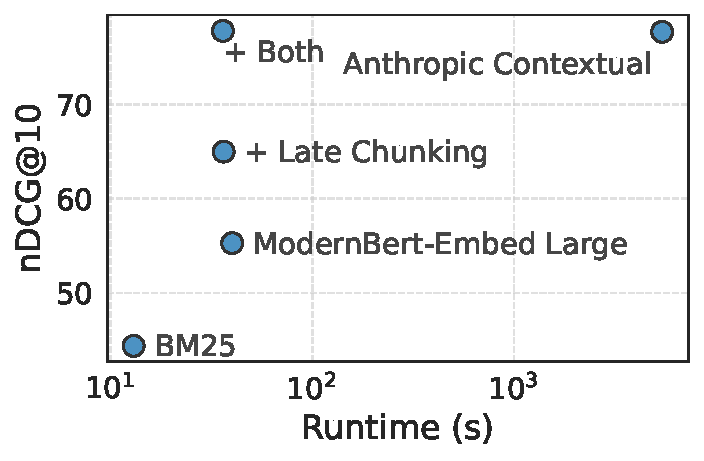
\includegraphics[width=\textwidth]{images/conteb_images/performance_vs_runtime.pdf}
%         \vspace{-3mm} % Reduce space between image and caption
%         % \caption{Retrieval performance vs. computational efficiency.}
%         \label{fig:pareto1}
%     \end{subfigure}
%     \hspace{1mm} % Reduce space between subfigures
%     \begin{subfigure}{0.49\textwidth}
%         \centering
%         \includegraphics[width=\textwidth]{images/conteb_images/lambda_seq.pdf}
%         \vspace{-3mm} % Reduce space between image and caption
%         % \caption{Alternative view of retrieval efficiency.}
%         \label{fig:pareto2}
%     \end{subfigure}

%     \vspace{-3mm} % Reduce space between subfigures and main caption
%     \caption{Side-by-side comparison of retrieval performance and computational efficiency. Our approach balances effectiveness and runtime optimally.}
%     \label{fig:pareto_combined}
% \end{figure*}

% Integrating conetxtual information makes a loagr diference (anthropoic contextual, both, and late chunking are largely ahead on all tasks, even wrt trained baseliens on the same data.


% Our training method unlocks extra performance, especiallu when it comes to integrating structuraml informatoip, (Insurance europa)

% our method is a the efficiency/performance frontier as shown in fig:pareto. While antrhopic's contextual yields slightly better performance, it requires expensive LLM summarization and contextualization which we do not require.

%
% \subsection{Not using doc wide context is suboptimal for retrieval}
\noindent\textbf{Document-wide context is essential.} As seen in \autoref{table:conteb:results}, methods leveraging contextual information widely outperform non-contextual methods across \emph{ConTEB} tasks. These results highlight the critical role of context-aware embeddings in improving retrieval performance in such settings, whether through untrained Late Chunking approaches or expensive context-aware reformulation approaches. 
As expected, the gap is even more notable in \emph{ConTEB}'s controlled setting experiments. 


% \textit{Our objective is to further boost the use of contextual clues through our training method to encourage improved information propagation across documents.} \manu{rework}


% \subsection{We can greatly improve upon existing contextualizations approaches with lightweight training}

% \noindent\textbf{In-Sequence Training.}
\noindent\textbf{Improving contextual information propagation.} Our results clearly show that \emph{InSeNT} variants outperform their untrained counterpart (+14.6 nDCG@10 for ModernBERT, +11.5 for ModernColBERT). Importantly, this is not due to the nature of the training data itself; the non-contextual ModernBERT model trained on the same data (ModernBERT + Training) does not improve upon the untrained baseline. Furthermore, the tasks that display the biggest improvements are the controlled setting tasks \textit{Insurance, Football}, that are explicitly designed to elicit information given in previous paragraphs, and that are out-of-domain w.r.t. our training set. 


\noindent\textbf{Late Interaction.} Interestingly, while LI models are good at long-context retrieving, they are poorly suited to out-of-the-box late chunking (-0.3 nDCG@10 w.r.t. ModernColBERT without LI). We posit that since token embeddings are never pooled, these models learn very local features and cannot leverage information from neighboring tokens. Once trained with our method, ModernColBERT+\emph{InSeNT} displays large performance gains across the board (+11.5 nDCG@10 w.r.t. ModernColBERT + Late Chunking), showcasing an increased ability to leverage external context.


\noindent\textbf{Context can add noise.} The \emph{CovidQA} task sticks out from the rest as untrained late chunking approaches severely degrade performance. Qualitative analysis, as well as the strong performance of the non-contextualized ModernColBERT method, indicate that the query-chunk pairing are often very extractive and match on technical medical terms, thus rendering context less useful. Our results show that naively applying late chunking in this setting adds noise and leads to notable performance drops (-21 nDCG@10), which are in large part recovered through our training method (+16 nDCG@10). 
%\manu{We perform toy viz to see this.}

% This indicates that the boosts achieved by through late chunking training are less about domain adaptation, and more about inducing meaningful information propagation between chunks. 

% To confirm performance gains in trained models are due to improved use of context rather than in-distribution training, XXX Trained on the exact same data, the non-contextual \textit{MB+Training} loses over 20 points to its contextual counterpart \textit{MB+InSeNT} on average.\manu{add details of this reference experiment to the appendix}

\begin{figure}[btp!]
    \centering
    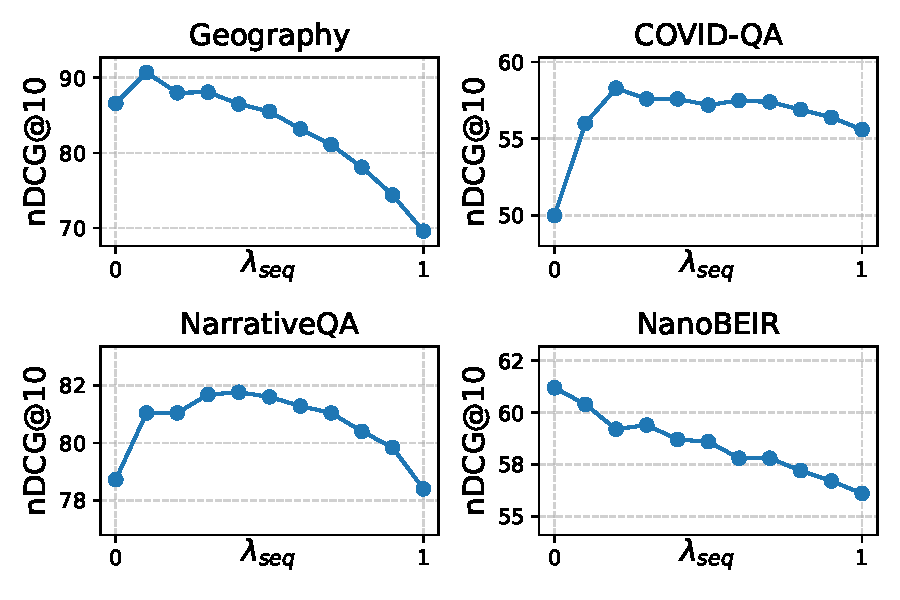
\includegraphics[width=0.65\textwidth]{images/conteb_images/lambda_seq_2x2.pdf}
    \caption[Importance of $\lambda_{seq}$]{\textbf{Importance of $\lambda_{seq}$}: Results for ModernBERT-Large trained with varying $\lambda_{seq}$. Optimal values depend on the task, but integrating both in-sequence and in-batch negatives is crucial to performance.}
    \label{fig:lambda_seq}
\end{figure}
\label{ablation_lambda_seq}

\noindent\textbf{$\lambda_{seq}$ matters.} The training objectives are to induce chunk representations to integrate document-level information (role of \emph{in-batch} negatives) while maintaining their specificity with respect to other same document chunks (role of \emph{in-sequence} negatives). By varying $\lambda_{seq}$ from \autoref{eq:loss_weighted}, we weight the importance of both objectives.

\noindent After training a series of models with varying $\lambda_{seq}$, we see on \autoref{fig:lambda_seq} that training with only in-sequence or in-batch negatives yields the worse results, and the optimal $\lambda_{seq}$ varies depending on the task. When documents need to be disambiguated between one another (\emph{NanoBEIR}, \emph{Geography}), up-weighting in-batch negatives seems optimal. On tasks where the challenge lies in locating information within a given document (\emph{NarrativeQA}, \emph{Covid-QA}), in-sequence negatives play a large role, but still need to be combined to in-batch negatives. Striking the optimal trade-off is thus very use-case dependent, and we opt for $\lambda_{seq}=0.1$ after tuning on the validation split of our training dataset.

% \textcolor{red}{These results interestingly build upon \sidecite{LateChunking}, highlighting the sensitivity of \textit{Late Chunking} to the weight of these joint objectives during training.}


% \noindent\textit{Our proposed training strategy improves upon LC by encouraging information propagation to favor inter-document separability (\emph{Football}, Geography), all the while limiting noise from the context, and making sure each document chunk embedding remains distinct from its neighbors (\emph{Insurance}, \emph{CovidQA}).} \manu{remove ? }\maxou{or move to conclusion}

\begin{figure*}
    \centering
    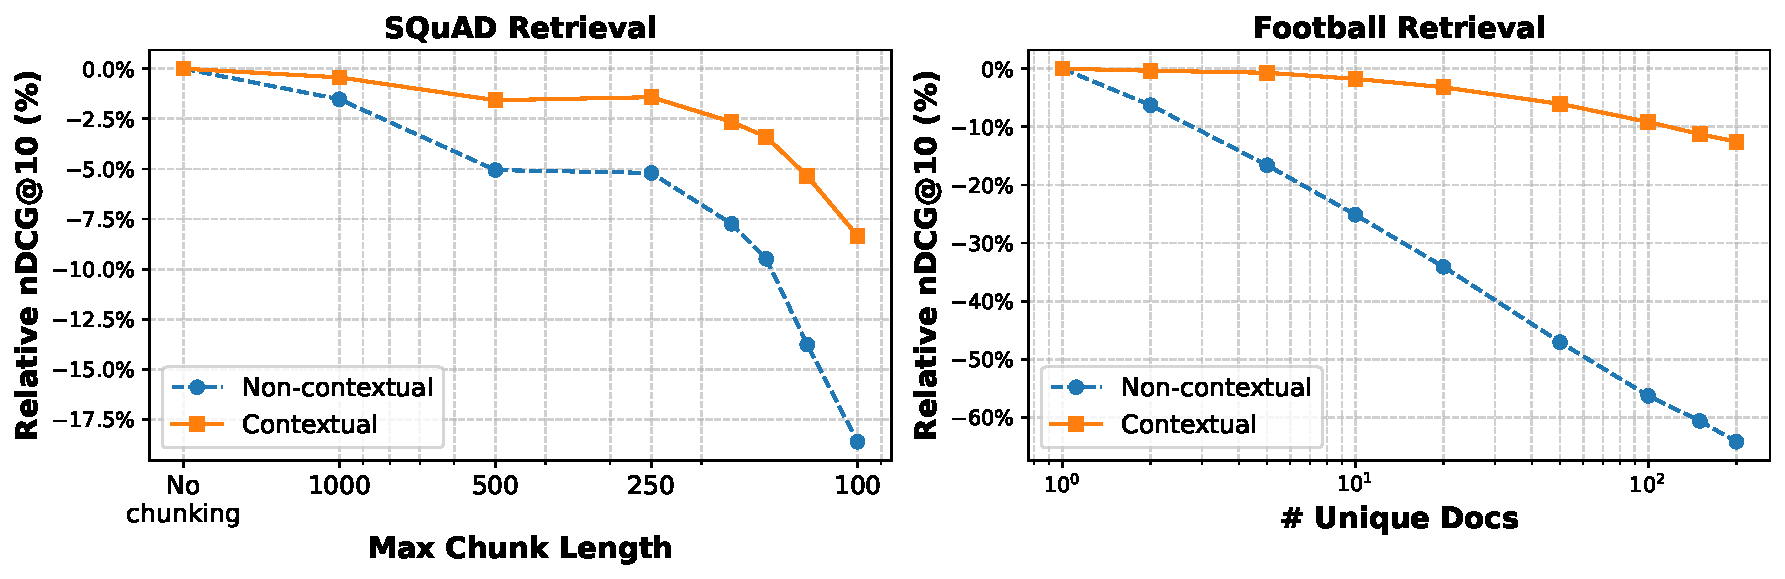
\includegraphics[width = 1\textwidth]{images/conteb_images/squad_football_retrieval.pdf}
    \caption[InSeNT robustness]{Contextualized models trained with InSeNT are more robust to aggressive chunking strategies that remove essential information from chunks (left), and scale better with corpus size and ambiguity (right).}
    \label{fig:robustness}
\end{figure*}


\noindent\textbf{Efficiency-Performance.} As shown in the Runtime column of \autoref{table:conteb:results}, our approach is very capable on contextual tasks, yet does not add much computational overhead. In fact, we find slight indexing speed improvements, attributed to our approach's reduced need for padding in-batch sequences of different lengths. While \textit{Anthropic Contextual} achieves sensibly similar performances on \emph{ConTEB}, it relies on costly LLM-based summarization and chunk reformulation, that are hardly scalable to huge corpora (120x slower).

\noindent\textbf{Short-Context Performance.} Careful hyperparameter tuning enables our best model to maintain strong performance on standard non-contextual benchmarks (\textit{NanoBEIR}), demonstrating that long-context optimization does not compromise short-context retrieval. Interestingly, LI models suffer from more degradation, which we posit is due to the original reliance on very local features modified through our training. Mixing in non-contextual "replay" data during training or merging models \sidecite{li2024improvinggeneraltextembedding_merging, modelmerging_lines} should further enable preserving the original embedding model's performances.

% \begin{figure}
%     \centering
%     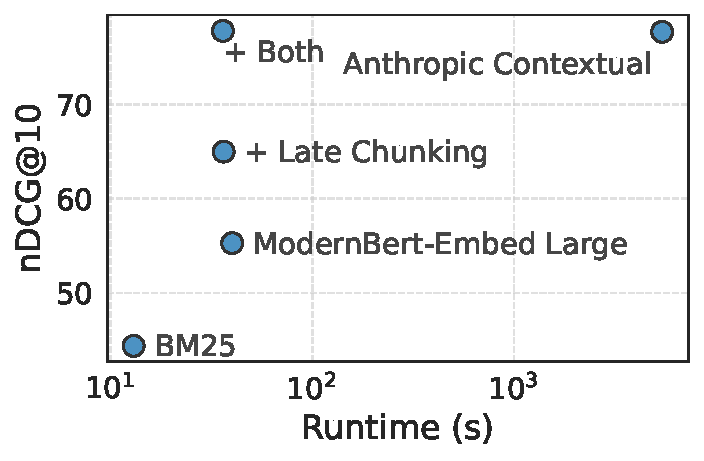
\includegraphics[width=0.45\textwidth]{images/conteb_images/performance_vs_runtime.pdf}
%     \caption{Comparison of retrieval performance versus computational efficiency across methods. Our approach achieves an optimal balance between effectiveness and runtime.}
%     \label{fig:pareto}
% \end{figure}


\section{Ablations}


% \noindent\textbf{Contextualized embedding training can be done without compromising the performance of the embedding model on short contexts}
% % our best models get better at long cxontext buyt stay good at beir. no tradeoffs !

% \noindent\textbf{Training on concatenated independent chunks hinders information propagation}
% % we train a model by concatenating short documents together from the nomic supervised dataset. we cluster these together as proposed by the paper cde-embeddings. We find evaluating these models on our benchmark severly degrases performance. Takeaway: essential to have long-context data that makes sense

% \noindent\textbf{The position in sequence matters}
% % evaluating if chunks in position 0 often have better representatioons  than later positionbs yierlds that yes. this is due to an encoder bis (needle in a haystackj). Takeaway: we must improve long context extension starategies in encoders to remove this bias (show this with nomic eval)


% \noindent\textbf{Preliminary contrastive finetuning with CLS token, then doing mean token pooling enable better transfer.}
% \section{Ablations}


% \subsection{\boldsymbol{\lambda_{seq}} matters.}

% \subsection{$\lambda_{seq}$ matters.}




\noindent\textbf{Robustness to chunking.}
We assess our method's robustness to poor chunking strategies using \emph{SQuAD} annotations.  Each originally self-contained chunk is split in multiple progressively smaller sub-chunks to while we keep track of the annotated answer span to identify the gold chunk. Eventually, these sub-chunks become too small to be self-contained and end up lacking sufficient information to be relevantly embedded on their own. \autoref{fig:robustness} (left) demonstrates that contextual embeddings greatly improves robustness w.r.t. suboptimal chunking. The model is able to elicit information from neighboring chunks to integrate contextual information within smaller sub-chunks, leading to a much more uniform retrieval performance across a wide range of chunk sizes.


\noindent\textbf{Robustness to corpus size.}
Common in the industry are templated documents that differ mostly by a key aspect (year, company name) but contain otherwise very similar information.
We study the dynamics of retrieval performance w.r.t. to the amount of similar documents in the corpus by computing scaling laws in which we iteratively vary the number of unique documents (composed of multiple chunks) in the corpus.
We observe in \autoref{fig:robustness} (right) that contextual embeddings scale vastly differently than their independently embedded counterpart. 
Intuitively, the greater the amount of similar documents and chunks in the corpus, the harder it is for a retrieval system to match the correct ones, but when embedding models are able to leverage external context, this effect is attenuated.



\noindent\textbf{Information Propagation.}
We experiment with concatenating semantically similar yet independent short chunks as "artificial" long documents. The resulting model is contextual as it uses late chunking, but exhibits performances in-line with non-contextual baselines (\textit{ModernBERT Large + Training}). We posit training on arbitrarily concatenated chunks, which by design are not contextually linked, teaches the model not to use information from neighboring chunks. This highlight the necessity of sourcing organic long-context data during training to induce correct training dynamics. Details in \autoref{table:nomic-results} in \autoref{app:res}.



% \subsection{Context-Aware chunks surpass Long-Context embeddings}

% \subsection{The Position in Sequence Matters}

% We investigate whether the position of a chunk in a sequence affects its representation quality. Our evaluation reveals that chunks appearing earlier in the sequence tend to have stronger representations compared to later ones. This bias is reminiscent of the \textit{needle-in-a-haystack} problem, where encoders struggle to maintain attention over longer spans. These findings indicate that current long-context extension strategies in encoders require further refinement to mitigate position-based biases. We illustrate this effect through evaluations on the \texttt{nomic} dataset.

% \subsection{Preliminary Contrastive Fine-Tuning with CLS Token, Followed by Mean Token Pooling, Enhances Transferability}

% \manu{See if useful} We experiment with a two-stage fine-tuning strategy: first performing contrastive learning using only the \texttt{[CLS]} token representation, followed by mean token pooling for final embeddings. This approach yields better transferability across retrieval tasks, as the initial contrastive step optimizes a global sequence representation before transitioning to a token-based aggregation strategy. Our results suggest that this hierarchical fine-tuning enhances generalization across both short and long retrieval tasks.


\section{Conclusions}
\label{section:conteb:conclusions_and_future_work}

In this work, we introduced \textit{ConTEB}, a benchmark designed to assess the effectiveness of retrieval models in leveraging document-wide contextual information. Our evaluation demonstrates that standard retrieval models struggle in context-dependent settings, while our proposed approach \textit{InSeNT}, which combines Late Chunking and a novel training methodology, performs strongly on \textit{ConTEB} without additional compute costs. % \textcolor{red}{These results prove the value of \emph{in-sequence} negatives in the training objective, and further bridge the gap towards practical utilization of the \textit{Late Chunking} paradigm.}
These insights build towards the broader development of the \textit{Late Chunking} paradigm in practice, and highlight the everlasting need for evaluation benchmarks that rigorously reflect how embedding models are used in real-world scenarios.
%By utilizing the ModernBERT architecture with late chunking and a weighted InfoNCE loss, we successfully integrate contextual knowledge into passage embeddings, leading to better retrieval performance with minimal computational overhead. 
% Our findings highlight the importance of contextual embeddings in enhancing retrieval accuracy, particularly in scenarios where document structure plays a crucial role.

\noindent\textbf{Future Work.} Scaling our approach with recent decoder models with extended context lengths (e.g., 1M+ tokens \sidecite{yang2025qwen251mtechnicalreport}) would enable embedding entire books or lengthy documents in a single forward pass, potentially unlocking new capabilities for large-scale document retrieval. It would also be interesting to observe the impact of our method on retrieval confidence \sidecite{gisserotboukhlef2024trustworthyrerankingsimpleeffective}. Finally, adapting our method to multi-modal embedding pipelines that have less control over the chunking strategy could further enhance retrieval systems in industrial applications with visually rich contextual documents \sidecite{faysse2025colpaliefficientdocumentretrieval, ma2024unifyingmultimodalretrievaldocument}. 
%Exploring new synthetic data generation strategies, and applying our training method with late interaction models \sidecite{khattab2020colbert} would also be an interesting avenue for future work.
% We hope our benchmark and findings serve as a foundation for future work in advancing context-aware retrieval systems.


% Talk about scaling this to decoders with 100K + token contexts. the vision is to emebd entire books in a single forward pass, this is a first step towards this vision. 
% another future step could be to apply this to embedding pipelines in which the system has less control on chunk construction, like page-level visual embeddings like colpali.


\section*{Limitations}

While our approach enhances retrieval performance in context-dependent settings, limitations persist.

\noindent\textbf{Context Length.} Our method is applied to long-context encoders that currently support sequences of up to 8k tokens. While we have shown performance can extrapolate to sequences of up to 32k tokens, scaling this approach to handle 1M+ token contexts with decoder-based models would be an interesting research avenue and presents significant compute and memory challenges. It notably requires rethinking the data construction processes to ensure longer documents are effectively leveraged.

\noindent\textbf{Non-contextual Performance.}
While our approach unlocks previously unattainable performance in contextual scenarios, it can come at the cost of slight short-context performance degradation. The optimal trade-off between non-contextual and contextual retrieval performance is highly usecase dependent \autoref{fig:lambda_seq} and can be parametrized by practitioners using the $\lambda_{seq}$ parameter. Other approaches may be promising such as model merging \sidecite{li2024improvinggeneraltextembedding_merging, modelmerging_lines}.


% \noindent\textcolor{red}{\textbf{Data Coverage.}
% While \textit{ConTEB} already covers a wide range of settings, we do believe there are still many avenues for future work. Increasing the language diversity (\textit{ConTEB} is English-only), integrating more domain-specific data with highly non-linear contexts (coding, legal texts) or experimenting with fixed context buffers (pre-pending Glossaries, or a List of Abbreviations, to texts) would further improve the coverage of contextual settings.}


\noindent\textbf{Data Generation.} The creation of training and evaluation data relies on existing datasets and semi-synthetic generation pipelines. However, a fully automated and scalable method for generating high-quality queries that effectively induce non-trivial context utilization remains an open challenge.

\noindent\textbf{Evaluation.} While our model demonstrates strong cross-domain performance, further validation in real-world applications, various use cases, and multiple languages is necessary to further assess its robustness and generalizability.

